\cotefile{150}
\scanpage{1}
\figure{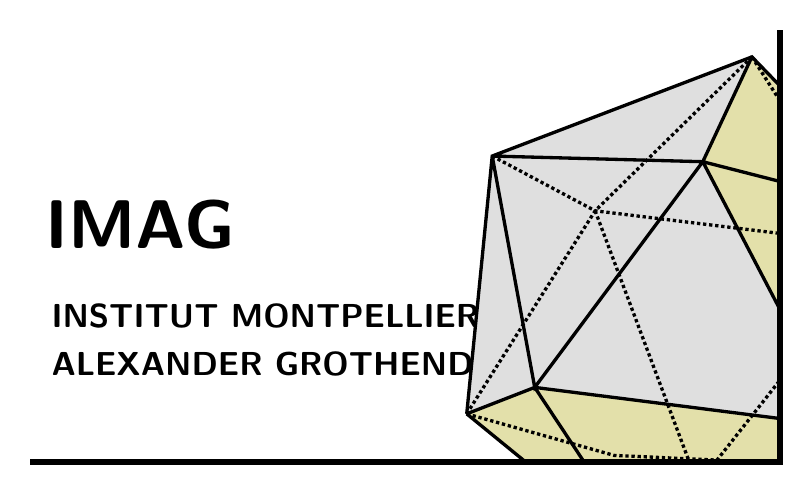
\begin{tikzpicture}[x=0.012cm,y=-0.012cm]
\node[anchor=west,font=\sffamily\bfseries\fontsize{80}{85}\selectfont] at (14,210) {IMAG};
\node[anchor=west,font=\sffamily\bfseries\large] at (20,306) {INSTITUT MONTPELLIERAIN};
\node[anchor=west,font=\sffamily\bfseries\large] at (20,357) {ALEXANDER GROTHENDIECK};
\fill[gray!25] (470,410)--(497,137)--(772,32)--(802,63)--(802,459)--(530,459)--cycle;
\fill[olive!25] (720,143)--(772,32)--(802,63)--(802,300)--cycle;
\fill[olive!25] (470,410)--(542,382)--(802,415)--(802,459)--(530,459)--cycle;
\draw[line width=1.2pt] (470,410)--(497,137)--(772,32)--(802,63) (497,137)--(720,143)--(772,32) (720,143)--(802,164) (720,143)--(802,300) (497,137)--(542,382)--(720,143) (470,410)--(542,382)--(802,415) (470,410)--(530,459) (542,382)--(593,459);
\draw[densely dotted,line width=1.2pt] (497,137)--(606,195)--(802,219) (470,410)--(606,195)--(772,32) (606,195)--(705,459) (772,32)--(802,79) (470,410)--(626,454)--(735,459)--(802,374);
\draw[line width=2pt] (8,461)--(802,461)--(802,4);
\end{tikzpicture}}

\scanpage{2}
déc. 81--janv. 82

\uline{Espaces stratifiés et voisinages côniques}

(ou : \uline{déploiement} \uline{des espaces stratifiés})

\diagram{\begin{tikzcd}[row sep=large,column sep=large]
& \Sigma_{ik} \arrow[rr,hook] \arrow[dl,"(F_{ik})"'] && \Sigma_k & \\
\Sigma_i && \Sigma_{ijk} \arrow[ul,hook] \arrow[rr,hook] \arrow[dl] \arrow[ur,phantom,"\mathrm{cart.}"] \arrow[dr,phantom,"\mathrm{cart.}"] && \Sigma_{jk} \arrow[ul,hook] \arrow[dl,"(F_{jk})"] \\
& \Sigma_{ij} \arrow[ul,"(F_{ij})"] \arrow[rr,hook] && \Sigma_j &
\end{tikzcd}}

$(i<j<k)$
\[
\left\{\begin{array}{ll}
\Sigma_i\ \Sigma_j\ \Sigma_k &: \text{strates déployées}\\
\Sigma_{ij}\ \Sigma_{jk}\ \Sigma_{ik} &: \text{tubes de raccord}\\
&\text{des strates 2 à 2}\\
\Sigma_{ijk} &: \text{jonction en }i,j,k
\end{array}\right.
\]
fibres $F_{ij},F_{jk},F_{ik}$ : fibres de raccord
 des strates 2 à 2.

les flèches $\hookrightarrow$ sont bordantes

les flèches $\longrightarrow$ sont des fibrations \inserted{(propres)}
(cas \unsure{équisingulier})

($F_{ijk}$, fibré sur $F_{ij}$, fibre $F_{jk}$ : \unsure{fibro-jonction}
\unsure{en} $i,j,k$

$\Sigma_i$ est la strate \inserted{déployée} ``âme'' du tube de raccord $\unsure{\Sigma_{ij}}$

$\Sigma_j$ en est la strate déployée ambiante

Cas non singulier : a) $\Sigma_i$ variété à bord, dont le bord est
la réunion des $\Sigma_{ji}$ $(j<i)$

b) $\Sigma_{jk}\longrightarrow\Sigma_k$ fibration : fibres des
variétés à bord \inserted{compactes}, le fibré des bords est
la réunion des $\Sigma_{ijk}$ pour $i<j<k$.

Plus généralement : a) $\Sigma_{i_0i_1\ldots i_n}=\Sigma_d$ est une
variété à bord, dont le bord est la réunion des
$\Sigma_{d'}$, avec $d'$ drapeau $\supset d$, cofinal à $d$
(il suffit de les prendre de la forme $d'=d\cup\{j\}$,
avec $j\in I_{<i_0}\amalg I_{i_0<\cdot<i_1}\amalg\cdots\amalg\unsure{I_{i_{n-1}<\cdot<i_n}}$)

b) $\Sigma_{i_0\ldots i_n}=\Sigma_d\longrightarrow\Sigma_{i_0\ldots i_p}=\Sigma_\delta$
est \unsure{fibrant|fibré}, à fibres des variétés à bord compactes,
le fibré des bords est réunion des $\Sigma_{d'}$
avec $d'\supset d$, $d$ cofinal dans $d'$, $\delta$ segment \unsure{initial}
de $d'$ -- il suffit de prendre $d'=d\cup\{j\}$, avec
$j\in I_{i_p<\cdot<\unsure{i_{p+1}}}\amalg\cdots\amalg I_{i_{n-1}<\cdot<i_n}$.

\mspage{1}

\scanpage{3}
\mspage{1}

$X$ espace topologique $\Longrightarrow$ \inserted{pré}ordonné par \uline{spécialisation} : $\unsure{\operatorname{Ord}(X)}$
\[
x\leq y\quad\overset{\mathrm{déf}}{\Longleftrightarrow}\quad\overline{\{x\}}\subset\overline{\{y\}}
\]
(ordonné ssi $X$ satisfait l'axiome de séparation $(T_0)$)

$I$ ens \inserted{pré}ordonné $\Longrightarrow$ espace top., fermés les $A\subset I$ t.q. $x\in A,y\leq x\Rightarrow y\in A$
ouverts les ens. fermés dans $I^\circ$ (opposé à $I$)
base d'ouverts : les ens $I_{\geq x}=\widetilde{\{x\}}$ ($\sim$ désigne l'adh. pour $I^\circ$)
\[
\operatorname{Esp}(I)
\]
\margin{\deleted{\unsure{lien foncteurs}}}

\uline{NB1} : Si $I,J$ préordonnés, $f:I\longrightarrow J$
une application, alors $f$ croissante ssi
$f$ continue.
\[
\overline{\{x\}}=I_{\leq x}=\{y\in I\mid y\leq x\}\qquad
\begin{aligned}
\text{donc }x\leq y&\Longleftrightarrow\overline{\{x\}}\subset\overline{\{y\}}\\
&\Longleftrightarrow x\in\overline{\{y\}}
\end{aligned}
\]
\inserted{Plus gén. $I\longrightarrow X$ continue ssi elle est croissante}
\margin{\deleted{\unsure{lien}}}

\uline{NB. 2} Une topologie sur un ens $I$ est associée à
un préordre (\unsure{néc.} unique, \unsure{ce sera celui de}
la spécialisation) ssi les réunions quelc. de
fermés sont fermés $\Longleftrightarrow$ intersections d'ouverts
sont ouverts (i.e. $\exists$ une ``topologie opposée'' !)

\unsure{Ceci} : deux foncteurs
\diagram{\begin{tikzcd}[column sep=large]
\mathcal E=(\operatorname{Esp}) \arrow[r,shift left,"\operatorname{Ord}"] \arrow[d,phantom,"\in"{rotate=90}] & (\operatorname{Préord})=\mathcal O \arrow[l,shift left,"\operatorname{Esp}"] \arrow[d,phantom,"\in"{rotate=90}]\\
X & I
\end{tikzcd}}
avec
\[
\operatorname{Ord}\circ\operatorname{Esp}=\operatorname{id}_{\unsure{\mathcal E}}
\qquad
\operatorname{Esp}\circ\operatorname{Ord}\longrightarrow\operatorname{id}_{\unsure{\mathcal O}}
\]
car l'application $\operatorname{id}_X:X\longrightarrow X$
est continue de $\operatorname{Esp}\operatorname{Ord}X$
dans $X$ (et est $\simeq$ ssi $X$
satisfait la cond. du NB2
\[
\operatorname{Hom}_{\mathcal E}(\operatorname{Esp}(I),X)\xrightarrow{\sim}
\operatorname{Hom}_{\mathcal O}(I,\operatorname{Ord}(X))\qquad\text{adjonction}
\]
$I\longrightarrow X$ est continue ssi elle est croissante

Considérons maintenant $\varphi:X\longrightarrow I$, i.e. une pseudo-partition : $X=\bigcup_{i\in I}X_i^*$
(les $X_i$ mutuellement disjoints). \inserted{Posons $X_J^*=\varphi^{-1}(J)$.} \deleted{continue ssi}
$\varphi^{-1}(I_{\geq i})$ ouverts
 i.e. ssi les $X_{\widetilde i}^*=\bigcup_{j\geq i}X_j^*$ sont ouverts, i.e. ssi les
$X_{\complement\widetilde i}^*=\bigcup_{\substack{j\in I\\j\not\geq i}}X_j^*$
sont fermés. Il faut pour ceci que les
$X_i\overset{\mathrm{déf}}=X_{\overline i}^*=\bigcup_{j\leq i}X_j$
soient fermés, et cette condition est suffisante
si $I$ est fini (car tt fermé est alors $\bigcup$ finie de fermés de la forme $\overline i$)
plus généralement si $\varphi$ est ``loct. finie'' i.e. loc. à ens. de val. fini
(\uline{NB} Si $I'\subset I$, la top. de $I'$ associée au préordre induit est la top. induite
par $I$)

\margin{\deleted{\illegible{3} $\unsure{x\leq y}\Longleftrightarrow\overline{\{x\}}\subset\overline{\{y\}}$ \unsure{en}}}
\margin{* \unsure{comme on veut que la top.}
\unsure{quotient en $I$ implique} topo, la
question est mal posée -- plutôt :
quelles conditions supplémentaires sur
$\varphi$ i.e. les $X_i^*$ imposer pour
avoir unicité ?}

Dans quels cas l'\inserted{pré}\uline{ordre} de l'ens $I$ est-il déterminé
par l'application $\varphi$ i.e. la famille $(X_i)_{i\in I}$ (dans le
cas $\varphi$ continue) ? * \inserted{plus précisément par $(X_i^*)_{i\in I}$ donné}
\deleted{\illegible{3}}
quand \deleted{\unsure{tout}} existe-t-il un ordre sur $I$ qui rende $\varphi$
continue, et quand cet ordre est-il unique ?
Pour l'unicité, il est clair que si $X=\varnothing$ il
faut que $\operatorname{card}I\leq1$, et si $X\ne\varnothing$ que $\varphi$ soit
surjective i.e. les $X_i^*\ne\varnothing$. Supposons donc $\varphi$ surj. i.e.
$X_i^*\ne\varnothing$. On aimerait que la top. de $I$ soit la \uline{top.}
\uline{quotient} i.e. que $X_J$ fermé ssi $J$ fermé en $I$.
Cette topologie sur $I$ est bien telle que les réunions
de fermés est fermé \inserted{(cas $\varphi$ loc. finie)} donc est associée à un ens
\unsure{ordonné de} $I$. Pour cet ordre, on aura donc
$i\leq j$ ssi \deleted{$\unsure{x\in}$} $\forall J\subset I$ tel que $X_J^*$ fermé et $j\in J$, on
a $i\in J$. À quelles conditions cette préordre est-il
un ordre (NB ``en général'' ce préordre aura tte
\unsure{chance} d'être chaotique !) Il faut et s. que
les $\{i\}$ soient localement fermés dans $I$, ce
qui implique que les $X_i^*$ sont loct. fermés. \deleted{\unsure{D'ailleurs}}
\deleted{\unsure{réciproquement}} il f. et s. que \inserted{$\forall i\in I$} l'on ait \deleted{$\unsure{\{i\}}$}
$\{i\}=\overline i\cap\widetilde i$ ce qui équivaut à \deleted{$\unsure{\forall i\in I}$}
$X_{\overline i}^*\cap X_{\widetilde i}^*=X_i^*$,
où $X_{\overline i}^*$ est le plus petit fermé de $X$ \inserted{$\supset X_i^*$} ``saturé'' par la
relation d'équivalence loc. finie assoc., et $X_{\widetilde i}^*$ est le
plus petit ouvert saturé $\supset X_i^*$. On pourrait appeler
une ``\uline{stratification fidèle}'' de $X$ une relation d'équiv.
loc\unsure{t.} finie telle que l'ens préordonné quotient
$I$ soit \uline{ordonné} -- ils correspondent à une famille
$(X_i^*)_{i\in I}$, partitions ensembliste de $X$ \inserted{indicée par $I$ ordonné}
\deleted{\illegible{4}} \unsure{tels que}
\unsure{disons et} telle que
Pour $J\subset I$, on ait $X_J$ fermé ssi $J$ fermé.
donc telle que a) les $X_i\overset{\mathrm{déf}}=\bigcup_{j\leq i}X_j^*$ fermés,
\inserted{i.e. $J$ fermé $\Rightarrow X_J$ est \unsure{fermé} ($\Rightarrow$ les $X_i^*$ loc. f.)}
b) Si $X_J$ est fermé, alors $J$ l'est.

\scanpage{4}
\mspage{3}

Condition plus forte : \deleted{\unsure{la topologie de $I$ est quotient pour}}
\inserted{(pour $\varphi$) l'application (continue \uline{surjective}) $\varphi$ est \uline{ouverte}}
\deleted{\unsure{celle de}}
\[
\deleted{\unsure{X_\varphi\text{ est fidèle}}}\quad\Longleftrightarrow\quad
\varphi^{-1}(\overline J)=\overline{\varphi^{-1}(J)}
\quad\Longleftrightarrow\quad
\varphi^{-1}(\overline j)=\overline{\varphi^{-1}(j)}\quad\text{i.e.}
\]
\[
\begin{array}{cc}
\Vert&\Vert\\
\displaystyle\bigcup_{j\in\overline J}X_j^*&
\displaystyle\overline{\bigcup_{j\in J}X_j^*}=\bigcup_{j\in J}\overline{X_j^*}
\end{array}
\]
\[
\overline{X_j^*}=\bigcup_{i\in\overline j}X_i^*\ (\overset{\mathrm{déf}}=X_j).
\]

Conditions pour une pseudo-partition $(X_i^*)_{i\in I}$ \inserted{\uline{loc. finie}} indexée par un ens
\uline{préordonné} $I$, i.e. $\varphi:X\longrightarrow I$ application, en supposant $\varphi$ \uline{continue}
\deleted{que} les $X_i=\bigcup_{j\leq i}X_j^*$ fermés (donc les $X_i^*$ loc. fermés)

\unsure{2°|4°}) Top. de $I$ est finale pour $\varphi$ (i.e. quotient si $\varphi$ surjective) $\Longleftrightarrow$
\[
(X_J^*\text{ fermé}\Rightarrow J\text{ fermé})\Longleftrightarrow
(X_L^*\text{ ouvert}\Rightarrow L\text{ ouvert})
\]
\margin{si $\varphi$ surj. i.e. 1° $\Uparrow$}

3°) $\unsure{\overline{X_j^*}|\overline{X_i^*}}=\bigcup_{j\leq i}X_j^*$ pour tt $\unsure{j|i}\in I$ i.e. $\varphi$ est ouverte

1°) $\varphi$ surj i.e. les $X_i^*\ne\varnothing$

\margin{\uline{NB} Moyennant 1°, 3°, on
récupère l'ordre de $I$ comme
la rel\unsure{ation} d'inclusion entre les
$\overline{X_i^*}$ \ldots}

\unsure{La donnée} $(X_i^*)_{i\in I}$ satisfaisant 1°) et 3°) équivaut à
\unsure{une} : une relation d'équiv. \uline{loc\unsure{t.} finie} et \uline{ouverte}
\deleted{\unsure{telle que les classes soient}}
et $I$ est l'espace quotient (avec la relation de \inserted{pré}ordre
de spécialisation), \deleted{\illegible{3}} l'ens $I$ est \uline{ordonné} ssi
\[
(\forall i,j\quad\overline{X_i^*}=\overline{X_j^*}\Rightarrow i=j)
\Longleftrightarrow(\text{les }X_i\text{ sont loc. fermés}).
\]

\margin{cas $I$ \uline{ordonné} $\Updownarrow$}
\uline{Stratification} \uline{\unsure{stricte}}

famille loc. finie \inserted{\uline{croissante}} $(X_i)_{i\in I}$ de fermés, telle que $\forall j<i$
implique que $X_j$ rare dans $X_i$, et $\forall i,j\in I$,
on ait
\[
X_i\cap X_j=\bigcup_{k\in\overline i\cap\overline j}X_k.
\]

Dans le cadre de la top. modérée, il faut voir \unsure{comment|au moins}
\inserted{pour} toute partition par des parties loc. fermées \uline{modérées},
il existe une plus petite \inserted{stratification en des parties}
\deleted{\unsure{partition finie}} \unsure{telle} qui
\deleted{\unsure{engendre}} la partition donnée.

\mspage{4}
\margin{\diagram{\[\begin{array}{cc|cc}
\subset\Rightarrow\times&\times\Rightarrow\subset&\subset&\subseteq\\
\unsure{\cap}&\uparrow&&\\
&\subset&&
\end{array}\]}}

$(X_i^*)_{i\in I}$ une \inserted{partition indexée} \deleted{famille} \inserted{de $X$}
\deleted{(loc. finie de parties disjointes de $X$,
de réunion $X$, donc \unsure{une} $X\xrightarrow{\varphi}I$)}. Cond. équiv.

a) $\forall i\in I$, \deleted{les $X_i^*\ne\varnothing$ (i.e. $\varphi$ surj, i.e. une partition), et}
$\overline{X_i^*}$ est saturé \deleted{\unsure{pour les $X_i^*$, loc. fermés}}

b) $\exists\leq$, une \deleted{relation} \inserted{pré}ordre sur $I$, telle que l'on ait $\forall i\in I$
\[
\overline{X_i^*}=\bigcup_{j\leq i}X_j^*
\]
(cette \deleted{relation} préordre est unique, \ldots
\[
i\leq j\Longleftrightarrow\overline{X_i^*}\subset\overline{X_j^*}
\quad(\Longleftrightarrow X_i^*\subset\overline{X_j^*})\ )
\]
c) La top. quotient de $I$ est telle que $\varphi:X\longrightarrow I$ soit ouverte,

i.e. $\forall U\in\operatorname{Ouv}(X)$, le saturé est ouvert

Sous ces conditions, la top. quotient de $I$ est bien
associée à \deleted{\unsure{sa relation d'ordre}} préordre, qui est aussi
la relation de spécialisation pour cette topologie.
Pour que $I$ soit ordonné, il f. et s. que les
$X_i^*$ soient loct. fermés. On dit alors que la partition est
\deleted{\unsure{stratifiée}} \unsure{(i.e. les $X_i^*$ saturés)}.
\inserted{\unsure{loc. finie}, pièces loc. fermées, relation d'équiv. ouverte}

On a une \uuline{correspondance} 1--1 entre les partitions
\inserted{\uline{stratifiantes}} de $X$ de cette forme, i.e. les relations d'équiv. loc.
finies et ouvertes, \inserted{sur $X$, à fibres loc. fermées}, et les familles (à iso près)
$(X_i)_{i\in I}$ indexées par un ens. d'indices $I$ \uline{ordonné}
\inserted{\uline{loc. fini}},
qui sont telles que 1°) familles \uline{croissantes} de parties
\inserted{\uline{fermées}} \deleted{\unsure{croissantes}} de $X$, \uline{recouvrant} $X$, et 2°) $\forall i,j\in I$
\[
X_i\cap X_j=\bigcup_{k\in\overline i\cap\overline j}X_k
\]
4°) \deleted{$\unsure{X_\alpha}$} $\forall i,j\in I$, $j<i$
$\Longrightarrow$ \inserted{$X_j$ rare dans $X_i$}
\deleted{\unsure{(telle que $X_i^*=X_i$)}}

3°) $\forall i$, $X_i^*\ne\varnothing$
\inserted{``déf'' $X_i\setminus\bigcup_{j<i}X_j$}

\margin{\uline{NB} Moyennant \unsure{1°}, 2°, 4°, 3° équivaut à
\unsure{la cond. plus faible}
3° bis $(\forall i\in I)$ $\unsure{X_i}\ne\varnothing$.}

Moyennant 1°) et 2°), en posant $X_i^*=X_i\setminus\bigcup_{j<i}X_j^*$,
les $X_i^*$ forment une ps. partition \inserted{\uline{loc. finie}} de $X$ par des
ens. loc. fermés, celle-ci satisfait les conditions
d'une \uline{partition} \uline{stratifiée} \uline{stricte} \inserted{(avec l'ordre donné de $I$)} ssi
on a 3°) et 4°).

\uline{Stratification} : Conditions \unsure{2°) et 1°)}. \uline{Strat. stricte} : ``fidèle'' (i.e.
3°) et condition de densité (4°) : \unsure{Partitions stratifiées} $\Longleftrightarrow$ \unsure{strat. strictes}

\margin{3}

\scanpage{5}
$\varphi:X\longrightarrow Y$\qquad $\varphi$ ouvert $\overset{\mathrm{déf}}\Longleftrightarrow$ ($U$ ouvert de $X\Rightarrow\varphi(U)$ ouvert)
\[
\Longleftrightarrow\deleted{\unsure{\forall}}\ (\forall B\subset Y,\quad\varphi^{-1}(\overline B)=\overline{\varphi^{-1}(B)})
\qquad(\text{NB c'est héréditaire})
\]
i.e. $\forall x\in X$, $\varphi(x)\in\overline B\Rightarrow x\in\deleted{\unsure{\varphi^{-1}}}\overline{\varphi^{-1}(B)}$
i.e. $\forall\underset{\mathrm{ouv.}}{U}\ni x$, $U\cap\varphi^{-1}(B)\ne\varnothing$ i.e.
\[
\forall U\in\operatorname{Ouv}(x),\quad\varphi(U)\cap B\ne\varnothing
\qquad\text{i.e. }\forall(B\in\mathcal P(Y),x\in X,U\in\operatorname{Ouv}_x(X),)
\]
\[
\varphi(x)\in\overline B\Rightarrow\varphi(U)\cap B\ne\varnothing\quad\text{i.e.}\quad
\forall(U\in\operatorname{Ouv}(X))\ \forall(y\in\overset{V=}{\varphi(U)}\subset Y),
\]
\[
y\in\overline B\Rightarrow V\cap B\ne\varnothing\quad\text{i.e.}\quad
\underbrace{V\cap B=\varnothing}_{B\subset X\setminus V}\Rightarrow\overline B\not\ni y
\]

5) Les conditions 1° et 2°) sont stables par image inverse
par $X'\longrightarrow X$, mais pas 3°) bien sûr (pas $=$ pour
un plongement ouvert), ni 4°) (mais au moins
4°) est stable par induction sur un ouvert). Les
relations d'équivalences ouvertes, par contre, s'indui-
sent bien sur un ouvert (mais on rapetisse $I$
en principe). \deleted{Admettons que \unsure{l'on ait pris la même}
\unsure{pour l'un et} 1°, 2°, 3° bis, \unsure{et alors} $\forall i,j\in I$, $X_i\subset X_j$
$\Rightarrow i\leq j$}
La condition \inserted{3° bis (en présence de 1° et 2°)}
implique la ``fidélité'' : $X_i\subset X_j\Rightarrow i\leq j$ (i.e. l'
ordre de $I$ est l'inclusion des $X_i$). \deleted{$I$ \unsure{l'inclusion}}
\deleted{\unsure{Si on a la fidélité, au contraire,} $X_i^*=\varnothing$ i.e. $X_i=\bigcup_{j<i}X_j$}
n'est pas vrai, exemple $I=$
\diagram{\begin{tikzcd}[column sep=small,row sep=small]
\deleted{\unsure{\bullet}} \arrow[dr,"\deleted{\unsure{\phantom{a}}}"',dashed] && c &\\
& \deleted{\unsure{\bullet}} & a \arrow[u] & b \arrow[ul]
\end{tikzcd}}
$X_c=X=X_a\amalg X_b$, \deleted{\unsure{tous les}} avec $X_a,X_b\ne\varnothing$, alors \unsure{on a}
fidélité, \inserted{les $X_i\ne\varnothing$,} mais $X_c^*=\varnothing$.

On suppose désormais 1°) 2°) 3° bis). Si $U\subset X$
est ouvert, les \inserted{$i\in I$ tels que} $X_i\cap U=U_i$ \deleted{tels que} \inserted{$\ne\varnothing$} forment un
ouvert $I_U$ de $\unsure{U|I}$, et $(U_i)_{i\in I_U}$ est une
stratification \deleted{ps.}fidèle de $U$. (Si on part d'une
stratification stricte, on aura une stratification
stricte de $U$). Ainsi, les strat. ps. fidèles des
ouverts de $X$ forment un préfaisceau, dont les
sections sont appelées les stratifications locales
\margin{\unsure{des}}

\deleted{Supposons} \inserted{Soit} $J$ tel que $X_J$ fermé, $J$ non fermé. \inserted{Supposons $J$ minimal}
\deleted{Donc $\exists j\in J$ tel que
$\overline j\not\subset J$. Soit $j$ minimal parmi ces éléments \unsure{de $I$}}
$j\in J$, $\overline j\not\subset J$, et $i<j$, $\Longrightarrow i\in J\Rightarrow\overline i\subset J$,
\deleted{\unsure{Plus généralement}} \uline{Soit}
\deleted{$\unsure{J\setminus J}=\unsure{\{j\}}\cup\bigcup i$}
$\unsure{J'_1}=\overline j\cap J$, donc $X_{\unsure{J'_1}}^*=X_{\overline j}^*\cap X_J^*$
\deleted{est fermé, donc que $J'$ n'est pas fermé. $J'$ \unsure{un}}

parmi de tels $J$ (on suppose $I$ fini, \unsure{un segt fini|un segment fini}\inserted{$\subset I$}) \unsure{l'on|l'un}
pour tt $K\subset I$, $K$ fermé et $K\cap J$ non fermé, \ldots $K\supset J$.
En particulier, $\forall j\in J$ tel que $\overline j\not\subset J$, \ldots $J\subset\overline j$
i.e. $j$ est plus grand él. de $J$. Donc $J$ a un plus grand
él. $j_0$, tel que pour tt autre élément \inserted{$j'$} de $J$, on ait
$\overline{j'}\subset J$. Donc \deleted{$\unsure{J}$}
$J_0=J\setminus\{j\}=\bigcup_{j'\in J\setminus\{j\}}\overline{j'}$ est fermé.
Donc $J=J_0\cup\{j\}$, $J_0$ fermé, $J_0\subset\overline j$, $j\notin J_0$
$\exists i\in\overline j\setminus J_0$ avec $i<j$. \deleted{$i\in\unsure{\overline j\cap I}$} On a donc
\[
X_J^*=X_{J_0}^*\cup X_j^*\quad(\text{réunion disjointe})
\]
qui est fermé, d'où
\[
X_j^\circ\overset{\mathrm{déf}}=\overline{X_j^*}\setminus X_j^*\subset X_{J_0}^*=X_{J_0}=\deleted{\unsure{\mathrm{ens}}}\bigcup_{i\in J_0}X_i,
\]
sans qu'on ait
pour autant $\overline j\subset J_0\cup\{j\}$.

Soit $I'$ une partie \uline{fermée} de $I$, minimale pour la
propriété : $\exists J\subset I'$, $J$ non fermé, avec $X_J$ fermé. Soit, pour
$I'$ fini, $J$ une \deleted{\unsure{partie}} de $I'$ minimale pour les propriétés précédentes,
On a donc $J\ne\varnothing$ et $J=J_0\cup\{j\}$, \deleted{$\unsure{\exists}$} $J_0$ fermé, $j\notin J_0$,
\deleted{$\unsure{\overline j\not\ni i}$} $J\subset\overline j$, $\overline j\not\subset J$ ceci, i.e. l'inclusion
\[
J=J_0\cup\{j\}\subset(\underbrace{J_0}_{\subset\overline j}\cup\overline j=\deleted{\unsure{\overline j}}\overline j)
\]
est stricte. \deleted{\unsure{de $I'$}} Pour tte
partie. Comme \inserted{\unsure{tt}} $\overline J\setminus\{j\}$ est encore fermé, d'après la condition
minimale de $I'=\overline J$ il s'ensuit que pour
 tt $J'\subset I'\setminus\deleted{\unsure{\{i\}}}\{j\}$, $X_{J'}^*$ fermé $\Rightarrow J'$ fermé. \deleted{\unsure{En}}

\figure{\begin{tikzpicture}[x=0.36cm,y=0.36cm]
\foreach \x/\y in {0/0,1/0.3,1.5/-0.3,2/0.8,2.5/0.3,3/0.8,4/0.5,4.5/1.6,5.5/1.4,5.2/0.5,6/0.9,7/0.8,7.2/0.2,8/0.4,8.6/0,9/-0.3,9/0.3}{\fill (\x,\y) circle (0.07);}
\draw plot[smooth cycle] coordinates {(4,1.8) (4.7,2.1) (5.8,1.6) (6,1.1) (5.6,0.9) (5.6,0.3) (4.7,0.4) (4.4,0.9) (4,1.2)};
\node at (6.6,1.8) {$j$};\node at (-0.5,-0.5) {$J_0$};
\end{tikzpicture}}

\deleted{particulier, pour tte partie fermée}
Conditions équiv.

a) $X_J^*$ fermé $\Rightarrow J$ fermé

b) $X_L^*$ ouvert $\Rightarrow L$ ouvert

c) $(\underbrace{X_j^\circ\overset{\mathrm{déf}}=\overline{X_j^*}\setminus X_j^*\subset X_{J_0},\ J_0\text{ fermé}}_{X_{J_0\cup\{j\}}^*\text{ fermé}})
\Rightarrow\overline j\subset J_0\cup\{j\}$
(i.e. $J_0\cup\{j\}$ fermé)
(\uline{NB} \unsure{ssi} $J_0\subset\overline j$), et pour \unsure{tout}
$J'\subset\overline j\setminus\{j\}$, $X_{J'}^*$ fermé $\Rightarrow J'$ fermé

\margin{4}

\scanpage{7}
\mspage{5}

\figure{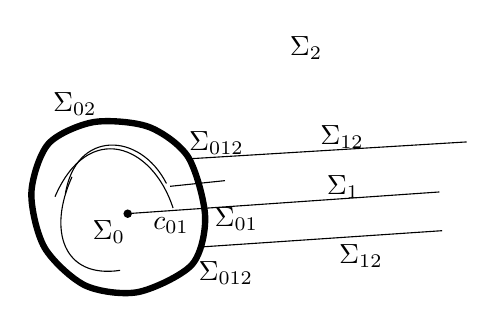
\begin{tikzpicture}[x=0.012cm,y=-0.012cm]
\draw[line width=2.3pt] plot[smooth cycle] coordinates {(267,310) (285,258) (333,235) (391,240) (433,272) (451,335) (437,386) (380,415) (324,408) (281,368)};
\draw (303,311) .. controls (314,243) and (382,245) .. (410,300);
\draw (292,314) .. controls (327,233) and (395,258) .. (417,326);
\draw (310,293) .. controls (284,350) and (301,401) .. (361,392);
\draw (414,303)--(472,297) (432,274)--(728,256) (368,332)--(699,309) (450,367)--(702,350);
\fill (369,332) circle (4.5);
\node at (558,157) {$\Sigma_2$};\node at (313,216) {$\Sigma_{02}$};
\node at (463,257) {$\unsure{\Sigma_{012}}$};\node at (596,251) {$\Sigma_{12}$};
\node at (349,351) {$\Sigma_0$};\node at (415,345) {$\unsure{c_{01}}$};
\node at (484,338) {$\Sigma_{01}$};\node at (597,304) {$\Sigma_1$};
\node at (473,395) {$\Sigma_{012}$};\node at (616,377) {$\Sigma_{12}$};
\end{tikzpicture}}
\margin{$\unsure{3}\quad\unsure{\uparrow}$}

\figure{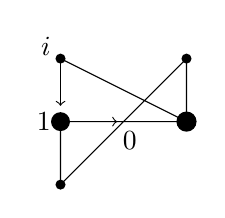
\begin{tikzpicture}[x=0.8cm,y=0.8cm]
\draw (0,2)--(2,1)--(2,2)--(0,0)--(0,1)--(2,1);
\draw[->] (0,2)--(0,1.25);\draw[->] (0,1)--(0.9,1);
\foreach \x/\y in {0/0,0/2,2/2}{\fill (\x,\y) circle (0.08);}
\fill (0,1) circle (0.15);\fill (2,1) circle (0.16);
\node[left] at (0,2.2) {$\unsure{i}$};\node[left] at (0,1) {$1$};\node[below] at (1.1,1) {$0$};
\end{tikzpicture}}

$\Sigma_{i_0i_1\ldots i_n}$\qquad\deleted{\unsure{covariant}} foncteur contravariant
par rapport aux drapeaux
variables $(i_0,\ldots,i_n)$
\[
\Sigma_i=X_i'=X_i\setminus\left(X_i\cap\bigcup_{k<i}\unsure{\mathring{\operatorname{Tub}}}(X_k,X_i)\right)
\]
\[
\Sigma_{(i,j)}=\deleted{\unsure{\partial}}\operatorname{Tub}^{\unsure{\bullet|\circ}}
\left(X_i',X_j\deleted{\unsure{\varnothing}}\setminus
\bigcup_{\substack{\deleted{\unsure{k<j}}\\\deleted{\unsure{k\ne i}}\\\inserted{i<k<j}}}
\operatorname{Tub}(X_k,X_j)\right)\hookrightarrow X_j'=\Sigma_j
\]
\[
i<k<j
\]

\margin{\diagram{\begin{tikzcd}
\Sigma_\delta\arrow[r,hook]\arrow[d]&\Sigma_{\delta'}\arrow[d]\\
\Sigma_d\arrow[r,hook]&\Sigma_{d'}
\end{tikzcd}}
\diagram{\[\begin{array}{ccc}d&\supset&d'\\\cap&&\cap\\\delta&&\delta'\end{array}\]}
cofinaux
\diagram{\begin{tikzcd}\unsure{\bullet}\arrow[d]\\d'\end{tikzcd}}}

\deleted{$\Sigma_{i,j}=F$}
\diagram{\begin{tikzcd}[column sep=large]
\mathcal V_{ij}=\mathcal V(X_i^*,X_j)\setminus\displaystyle\bigcup_{i\leq k<j}\mathcal V(\unsure{X_i^*|X_i'},X_j)\cap X_k\arrow[r,hook]\arrow[d]&X_j^*\\
X_i^*&
\end{tikzcd}}
\[
X\qquad\mathcal V_{ijk}
\]
\diagram{\begin{tikzcd}[row sep=large,column sep=large]
\mathcal V_{ijk}\arrow[r]\arrow[d]&\mathcal V_{jk}\arrow[d]&X_k^*\arrow[l,hook]\arrow[d,"\unsure{\sim}"']\\
\mathcal V_{ij}\arrow[r,hook]\arrow[d]&\mathcal V(X_j^*,X_k)\arrow[r,"\deleted{\unsure{\sim}}"]&\deleted{X_k}\\
X_i^*&&
\end{tikzcd}}

\margin{$\lambda_i'T'=\lambda_i''T''$\qquad
$a\leq\operatorname{Inf}(\lambda_i',\lambda_i'')$}
\margin{6}

\scanpage{8}
$\Sigma_0,\Sigma_1,\Sigma_2$ espaces top.
\[
\Sigma_{01}\subset\unsure{\Sigma_{01}|\Sigma_0\times\Sigma_1},\quad
\Sigma_{12}\subset\Sigma_1\times\Sigma_2,\quad
\Sigma_{02}\subset\Sigma_0\times\Sigma_2\qquad\text{fermés}
\]
\deleted{\unsure{a)}} Posons
\[
\begin{array}{c}
\Sigma_{012}\subset\Sigma_0\times\Sigma_1\times\Sigma_2\\
\Vert\\
(\Sigma_{01}\times\Sigma_2)\cap(\Sigma_0\times\Sigma_{12})
\end{array}
\]
a) On veut que $\operatorname{Im}(\Sigma_{012}\longrightarrow\Sigma_0\times\Sigma_2)\subset\Sigma_{02}$

de sorte qu'on a un diagramme commutatif
\diagram{\begin{tikzcd}[row sep=large,column sep=large]
&\Sigma_{02}\arrow[r,hook]\arrow[dl]&\Sigma_2\\
\Sigma_0&\Sigma_{012}\arrow[l,"{[\ell]}"']\arrow[u,hook]\arrow[r,hook]\arrow[d,"{[\ell]}"]\arrow[ur,phantom,"\deleted{\mathrm{cart}}"]\arrow[dr,phantom,"\mathrm{cart}"]&\Sigma_{12}\arrow[u,hook]\arrow[d,"{[\ell]}"]\\
&\Sigma_{01}\arrow[ul,"{[\ell]}"]\arrow[r,hook]&\Sigma_1
\end{tikzcd}}
\margin{signifie que
sur $\Sigma_* = \Sigma_0\amalg\Sigma_1\amalg\Sigma_2$
on a une relation d'ordre
au dessus de $[0,1,2]$}

b) $\Sigma_{01}\longrightarrow\Sigma_1$, $\Sigma_{02}\longrightarrow\Sigma_2$, $\Sigma_{12}\longrightarrow\Sigma_2$ sont injectifs
(et \uline{bordants}) (donc $\Sigma_{012}\longrightarrow\Sigma_{12}$ aussi)
\deleted{\unsure{c)}} \inserted{donc aussi} $\Sigma_{012}\longrightarrow\Sigma_{\unsure{02|2}}$
\deleted{est injectif} \inserted{et a fortiori} (\deleted{$\unsure{\Longleftrightarrow}$} $\Sigma_{012}\longrightarrow\Sigma_{02}$).

c) \deleted{est injectif), et de plus}
On a $\Sigma_{012}=\Sigma_{02}\cap\Sigma_{12}$ dans $\Sigma_{12}$ i.e.
le carré sup. est aussi cartésien.

d) $\Sigma_{12}\longrightarrow\Sigma_1$ est transversal p.r. à
une inclusion bordante $\Sigma_{01}\longrightarrow\Sigma_1$. (Cela \unsure{sous que}
$\Sigma_{012}\longrightarrow\Sigma_{12}$ est aussi bordant)

e) $\Sigma_{02}$ et $\Sigma_{12}$ sont \inserted{parties bordantes} transversales dans $\Sigma_2$
(donc $\Sigma_{012}\hookrightarrow\Sigma_{02}$ est aussi bordant)

f) $\Sigma_{01}\xrightarrow{[\mathrm{liss}]}\Sigma_0$, $\Sigma_{02}\longrightarrow\Sigma_0$, $\Sigma_{12}\xrightarrow{[\mathrm{liss}]}\Sigma_1$ fibrant
(donc $\Sigma_{012}\xrightarrow{[\mathrm{liss}]}\Sigma_{02}$ fibrant, \deleted{\unsure{donc}} et $\Sigma_{012}\xrightarrow{[\mathrm{liss}]}\Sigma_{01}$ aussi)

\margin{f) \unsure{devrait se remplacer}, par
la condition que le diagramme
\diagram{\begin{tikzcd}\Sigma_{01}&\Sigma_{012}\arrow[l]\arrow[r]&\Sigma_{02}\end{tikzcd}}
au dessus de $\Sigma_0$
est loct. trivial sur $\Sigma_0$.}
\margin{7}

\scanpage{9}
\deleted{
\diagram{\[\begin{array}{l r c r c r c r}
\text{MM. Grothendieck}&10\ 200&+&-&+&212&=&10\ 412\\
\text{\phantom{MM. }Hakim}&10\ 200&+&-&+&212&=&10\ 412\\
\text{\phantom{MM. }Lefranc}&10\ 200&+&18\ 000&+&1\ 270&=&29\ 470\\
\text{\phantom{MM. }Lemaire}&10\ 200&+&13\ 680&+&1\ 227&=&25\ 107\\
\text{\phantom{MM. }Loupias}&10\ 200&+&-&+&423&=&10\ 623\\
\text{\phantom{MM. }Maisonneuve}&10\ 200&+&-&+&212&=&10\ 412\\
\text{\phantom{MM. }Micali}&10\ 200&+&27\ 000&+&1\ 799&=&38\ 999\\
\text{\phantom{MM. }Molino}&10\ 200&+&9\ 000&+&741&=&19\ 941\\
\text{\phantom{MM. }Moreau}&10\ 200&+&5\ 400&+&529&=&16\ 129\\
\text{\phantom{MM. }Nouazé}&10\ 200&+&3\ 600&+&423&=&14\ 223\\
\text{\phantom{MM. }Roby}&10\ 200&+&4\ 320&+&466&=&14\ 986\\
\text{\phantom{MM. }Roumieu}&10\ 200&+&6\ 120&+&571&=&16\ 891\\
\text{\phantom{MM. }Sabatier}&10\ 200&+&41\ 760&+&2\ 878&=&54\ 838\\
\text{\phantom{MM. }Valadier}&10\ 200&+&-&+&212&=&10\ 412\\
\cline{2-2}\cline{4-4}\cline{6-6}\cline{8-8}
&193\ 800&+&129\ 960&+&12\ 509&=&336\ 269
\end{array}\]}

\diagram{\[\begin{array}{l c r}
\text{Déficit 1979}&-&29\ 393{,}80\\
\text{Avance Bibliothèque}&-&10\ 000{,}00\\
\text{Crédit Installation M. Auberson}&+&10\ 000{,}00\\
\text{Crédit Dawson}&+&2\ 052{,}50\\
\cline{3-3}
&-&27\ 341{,}30\\[1em]
\text{Somme Crédits Recherche}&&\boxed{308\ 927{,}70}
\end{array}\]}

3°) \uline{D. E. A.} :
\diagram{\[\begin{array}{l r r}
\text{MM. Charles}&1\ 261{,}20&\\
\text{\phantom{MM. }Lemaire}&1\ 681{,}60&\\
\text{\phantom{MM. }Micali}&3\ 363{,}20&\\
\text{\phantom{MM. }Molino}&420{,}40&\\
\text{\phantom{MM. }Roumieu}&840{,}80&\\
\text{\phantom{MM. }Sabatier}&3\ 363{,}20&\\
\cline{2-2}
&10\ 930{,}40&\qquad\qquad10\ 930{,}40
\end{array}\]}
}
\margin{8}

\scanpage{10}
\figure{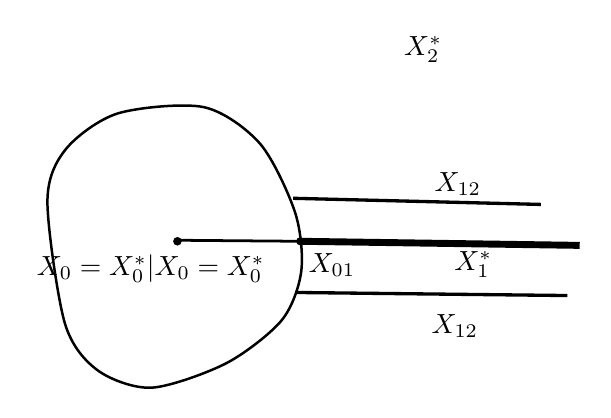
\begin{tikzpicture}[x=0.013cm,y=-0.013cm]
\draw[line width=0.9pt] plot[smooth cycle] coordinates {(336,220) (354,169) (405,134) (489,128) (544,164) (578,231) (584,288) (565,336) (511,378) (438,402) (385,385) (353,339)};
\draw[line width=1.2pt] (576,217)--(818,223) (578,309)--(844,312);
\draw[line width=1pt] (464,258)--(583,259);
\draw[line width=2.5pt] (583,259)--(856,263);
\fill (463,259) circle (4.2);\fill (583,259) circle (4);
\node at (703,72) {$X_2^*$};\node at (437,286) {$\unsure{X_0=X_0^*|\uline{X}_0=\uline{X}_0^*}$};
\node at (614,282) {$X_{01}$};\node at (737,203) {$X_{12}$};
\node at (752,282) {$\unsure{X_1^*}$};\node at (734,342) {$X_{12}$};
\end{tikzpicture}}
\margin{9}

\scanpage{12}
\mspage{1}
Espaces stratifiés (étude par voisinages \deleted{tubulaires}
\inserted{coniques})
\textcircled{I}

\textcircled{1} Soit $Y$ un espace topologique. Un \uline{voisinage \deleted{tubulaire}} \inserted{\uline{conique}}
\inserted{(\uline{``absolu''})} de \deleted{$Y$}
\inserted{(ou ``cône sur $Y$'')} est un espace topologique
$\bar T\deleted{\unsure{_Y}}$ contenant $Y$
(la ``\uline{base}''), muni d'une partie fermée $\dot T$
(le ``bord'' du tube'') et d'une opération du monoïde topologique
$I=[0,1]$ (pour la multiplication) sur $\bar T$, notée
\[
(1)\qquad (\lambda,t)\longmapsto\lambda t
\qquad I\times\bar T\longrightarrow\bar T
\]
satisfaisant :
\[
\begin{array}{ll}
a)&\lambda y=y\quad\forall y\in Y\\
b)&0.\deleted{\unsure{\bar T}}\bar T\subset Y
\end{array}
\]
\margin{donc les $\lambda_{\bar T}:\bar T\longrightarrow\bar T$
$(0\leq\lambda\leq1)$ forment une homotopie de
l'identité $\operatorname{id}_{\bar T}$ (pour $\lambda=1$)
sur une \uline{rétraction} de $\bar T$ sur $Y$,
laissant les pts de $Y$ fixes au cours de l'homotopie}
\margin{\uline{NB} La condition b) \unsure{sous sa forme faible}
$b')\ 0.\dot T\subset Y$, plus la condition c)
(\unsure{à qui celle-ci donne un sens}) suffisent :
\unsure{entraînent} (b).}

c) Le \deleted{application} diagramme d'applications
\diagram{\[
(2)\qquad
\begin{tikzcd}[column sep=large]
I\times\dot T \arrow[r,"{(\lambda,\unsure{x})\mapsto\lambda x}",
"\deleted{\unsure{g}}"'] & \bar T\\
\{0\}\times\dot T \arrow[u,hook] \arrow[r,"{(0,x)\mapsto0.x}"'] & Y \arrow[u,hook,"\mathrm{inc}"']
\end{tikzcd}
\]}
est \uline{cocartésien}$^{*}$, i.e. identifie $\bar T$ au cône de l'application
\[
(3)\qquad f:\dot T\longrightarrow Y\qquad f(x)=0.x
\]
\margin{$^{*}$ Cela signifie que
$]0,1]\times\dot T\xrightarrow[\sim]{\mathrm{bij.}}\bar T\setminus Y$
et qu'une partie de $\bar T$ est ouverte ssi
\deleted{\unsure{son intersection}} \inserted{\unsure{ses images}}
\unsure{dans $Y$ et ses images dans $I\times\dot T$}.}
\[
(4)\qquad \bar T\simeq C(f)
\]
Dans cette identification, $Y\hookrightarrow\deleted{\unsure{T}}\bar T
\hookleftarrow\dot T$ correspondent
aux applications canoniques \deleted{\unsure{du cône $f$}}
$\operatorname{but}(f)\hookrightarrow C(f)\hookleftarrow
\operatorname{source}(f)$
et l'opération de $I$ sur $\bar T$ provient de l'opération de
$I$ sur $C(f)$, définie par passage au quotient de
l'opération évidente de $I$ sur $I\times\dot T$, et l'op. triviale
de $I$ sur $Y$. Les axiomes a) b) c) signifient
aussi que la situation $(\unsure{Y-\bar T\longrightarrow\dot T},
\unsure{I\times\bar T-\bar T})$
est isomorphe à celle d'un $C(f)$ avec $f:\dot T\longrightarrow Y$.
Notons que $\dot T$ est \unsure{connu quand on connaît} l'opération
de $I$ sur $\bar T$, \deleted{\unsure{comme on}} et posons
\[
(5)\qquad \mathring T=\bar T\setminus\dot T
\quad\text{(l'\uline{intérieur} du tube)}
\qquad\text{et notons que }\mathring T=\bigcup_{\lambda\in[0,1[}\lambda\bar T
\]
\margin{11}

\scanpage{13}
\deleted{2. Soit $X$ un espace, $Y$ un sous-espace fermé.}
\deleted{$(\unsure{6})$ Soit $\bar T$}

\uline{NB} Les $\bar T_\lambda$ $(\lambda\in[0,1])$ forment
une famille croissante de parties fermées de
$\bar T$, les $\mathring T_\lambda\overset{\mathrm{déf}}=
\lambda\mathring T\deleted{\unsure{_\lambda}}$ $(\lambda\in]0,1])$
une famille croissante de parties ouvertes. Si $\lambda\in]0,1[$, alors
$\mathring T_\lambda$ est bel et bien l'intérieur \inserted{topologique}
de $\bar T_\lambda$ dans $\bar T$,
mais bien sûr $\mathring T_1=\mathring T$ n'est pas l'intérieur
\inserted{top.} de $\bar T_1$ dans
l'espace topologique $\bar T_1=\bar T$, i.e. on n'a pas
$\mathring T\deleted{\unsure{_1}}=\bar T$ sauf
si $\dot T=\varnothing$ i.e. $Y=\bar T$.

Posons, pour $\lambda\in]0,1[$
\[
(\unsure{6})\qquad
\left\{\begin{aligned}
\bar T\setminus\mathring T_\lambda
&\overset{\mathrm{déf}}=\deleted{\unsure{E}}
\mathrm{Ep}^{(T)}_{1-\lambda=\varepsilon}
\quad\text{``épaississement d'indice $\varepsilon$''}\\
&\hspace{4em}\text{du bord $\dot T$ de $\bar T$}\\
\dot{\mathrm{Ep}}_\varepsilon^{(T)}
&\overset{\mathrm{déf}}=\dot T\cup(1-\varepsilon).\dot T
\end{aligned}\right.
\]
\uline{NB} La frontière de $E_\varepsilon$ dans $\bar T$ est
$(1-\varepsilon)\dot T$, et $E_\varepsilon$
est un voisinage de $\dot T$. On a
\[
(7)\qquad\mathrm{Ep}_\varepsilon^{(T)}
\simeq[\underbrace{1-\varepsilon}_{\lambda},1]\times\dot T
\]
\margin{\uline{NB} Si $Y,\dot T$ \unsure{compacts}, \deleted{\unsure{les}}
alors $\bar T$ compact, et les $\bar T_\varepsilon$
$(\varepsilon\in]0,1\unsure{[|]})$ forment
un syst. fond. de voisinages de $Y$ dans $\bar T$,
\deleted{fermés}\inserted{\unsure{ouverts}}.
(\unsure{ainsi que voisinages} $\unsure{\bar T_\varepsilon}$ tubulaires absolus de $Y$)}

\textcircled{2} Soit $Y\hookrightarrow X$ une inclusion fermée d'espaces
topologiques. Un \uline{voisinage conique} de \uline{$Y$ dans} $X$
est un voisinage $\bar T$ de $Y$ dans $X$
muni d'une opération (1) $I\times\bar T\longrightarrow\bar T$
\inserted{faisant de $\bar T$ un vois. \deleted{tub.}\inserted{coniq.}
absolu de $Y$.} \deleted{satisfaisant les conditions id.}
Alors les
$\lambda\bar T=\bar T_\lambda$ $(\lambda\in]0,1])$
forment d'autres voisinages
tubulaires de $Y$ dans $X$ (famille croissante) et
on voit que pour $\lambda\in]0,1[$, on a
\[
(8)\qquad\dot T_\lambda=\lambda\dot T
\quad\text{est la frontière de }\bar T_\lambda=\lambda\bar T\text{ dans }X.
\]
\margin{12}

\scanpage{14}
\mspage{2}
Mais on ne peut pas dire \inserted{en général} que $\dot T$ soit la frontière
de $\bar T$ dans $X$, i.e. (\unsure{7|8}) devient faux si $\lambda=1$
(prendre $X=\bar T\deleted{\unsure{_\lambda}}$, avec $\dot T\neq0$).

\deleted{On dira} \unsure{que} dire qu'une partie fermée $\unsure{Y|Z}$ d'un
espace topologique $X$ est une ``\uline{partie bord}''
s'il existe un \uline{voisinage} \deleted{\uline{collier}}
\inserted{\uline{cylindrique}} de $\unsure{Y|Z}$ dans $X$,
i.e. un voisinage \deleted{tubulaire} conique $\bar T$ tel que
$\dot T\longrightarrow Y$ soit un homéom. --- ou ce qui revient
au même, \deleted{i.e. tel que l'on} s'il existe un
voisinage $\deleted{\unsure{de}}\bar T$ de $Y$ dans $X$ et un homéom.
\[
(9)\qquad\bar T\simeq Y\times I
\]
rendant commutatif le diagramme
\diagram{\[
(10)\qquad
\begin{tikzcd}
Y\arrow[r,hook]\arrow[dr,"{y\mapsto(y,0)}"']&\bar T\arrow[d,"\simeq",draw=none]\\
&Y\times I
\end{tikzcd}
\]}
\margin{définir la \unsure{structure} de voisinage cylindrique
comme un homéom.
$E\simeq Y\times[0,1]$
compatible avec
\diagram{\[
\begin{tikzcd}
Y\arrow[r]&\unsure{[0,1]|Y\times[0,1]}\\
y\arrow[r,mapsto]&(y,0)
\end{tikzcd}
\]}}

Par exemple, si $\bar T$ est un voisinage \deleted{tubulaire} conique
\inserted{(absolu)} de \deleted{\unsure{tout}} $Y$, alors $\dot T$ est un sous-espace bord.
\unsure{donc} $\unsure{\bar T_\lambda|\dot T_\lambda}$ est un sous-espace bord de $\bar T_\lambda$ ;
$\deleted{\unsure{\mathrm{Ep}}}\dot T,(1-\unsure{\varepsilon|\lambda})\dot T$
et $\dot T\cup(1-\varepsilon)\dot T$ sont des sous-espaces
bords de $\mathrm{Ep}_\varepsilon^{(T)}$. \deleted{Dans}
Si $X$ est un espace
\uline{compact}, et $(Y_i)_{i\in I}$ une \unsure{partie|famille} finie de
parties fermées disjointes de $X$, alors
$Y=\bigcup_{i\in I}Y_i$ est un sous-espace bord ssi les $Y_i$ le sont.
\margin{13}

\scanpage{15}
\deleted{On dit}\inserted{Soit} $\bar T$ un voisinage
\deleted{tubulaire}\inserted{conique} de $Y\subset X$
dans $X$, posons
\[
(11)\qquad X^*=X\setminus\mathring T=(X\setminus\bar T)\cup\dot T
\]
c'est une partie fermée de $X$. \deleted{On dit que}

\uline{Prop.} Conditions équivalentes (où $\lambda\in]0,1[$ donné)

a) $\dot T$ est une partie-bord de $X^*=X\setminus\mathring T$

b) Il existe un homéomorphisme de $X$
avec lui-$=$, transformant $\bar T,\dot T$ en
$\deleted{\unsure{\lambda}}(\bar T_\lambda,\dot T_\lambda)$

b') Comme b, mais en supposant de plus
que l'homéomorphisme induit l'identité
sur $\bar T_{\lambda'}$ (où \deleted{$0<\lambda'<\lambda$}
$\lambda'$ est donné, $0<\lambda'<\lambda$).

c) Il existe un voisinage \deleted{tubulaire} conique $\bar T'$
de $Y$ dans $X$, \deleted{tel que et \unsure{a}} tel que $\bar T=\lambda\bar T'$,
l'isomorphisme étant compatible avec les
structures de voisinages coniques.

On dit alors que $\bar T$ est un vois. \deleted{tub.} conique
\uline{strict} dans $X$.

\margin{Il vaut mieux de définir les voisinages coniques
stricts comme \unsure{des} \uline{germes} de voisinage
plus grand $(1+\varepsilon)\bar T\unsure{-R_{>0}}$
$(\varepsilon>0)$}

\uline{Corollaire} Quand $\bar T$ est vois. \deleted{tub.} con. strict dans $X$,
$\dot T$ est la frontière de $\bar T$ dans $X$.

\uline{Corollaire} Si \deleted{il est}\inserted{$\bar T$} voisinage
\deleted{tubulaire}\inserted{conique} de $Y$
dans $X$, les $\bar T_\lambda$ $(\lambda\in]0,1[)$ sont des voisinages
\deleted{tubulaires}\inserted{coniques} stricts.
\margin{14}

\scanpage{16}
\mspage{3}
\textcircled{3} Soit
\deleted{$X\supset Y$, $X$ muni de sous-espaces}
\inserted{$\bar T$ un vois. \deleted{tub.} conique absolu de $Y$.}
Soit $\bar T'\deleted{\unsure{_\varepsilon}}\subset\bar T$.
On dit que $\bar T'$ est \uline{sous-espace conique} dans $\bar T$ si on a
\[
(12)\qquad\left\{\begin{array}{ll}
a)&\bar T'\text{ stable par homothéties }\lambda\in I\
\deleted{\unsure{\lambda\bar T'\subset\bar T'}}\\
b)&\text{Pour cette opération, }\bar T'\text{ est un voisinage}\\
&\deleted{\text{tubulaire}}\text{ conique de }Y.
\end{array}\right.
\]
\uline{NB} On aura nécessairement $\dot T'=\bar T'\cap\dot T$,
$\bar T'_\lambda=\bar T'\cap\bar T_\lambda$ ;
\deleted{Si $(\bar T_i)_{i\in I}$ est une famille}
\inserted{la donnée de $\bar T'$ équivaut à}
celle d'un sous-espace fermé $\dot T'$ de $\dot T$
et d'un sous-espace $Y'$ de $Y$, tel que $Y'\supset0.\dot T'$, et
on a
\[
\bar T'=\operatorname{Im}(I\times\dot T'
\deleted{\unsure{_\lambda}}\longrightarrow\bar T)\cup Y'.
\]
\margin{On dit que $\bar T'$ est conique \uline{pur}
si $\bar T'\cap Y=0.\dot T'$,
--- \unsure{ces $\bar T'$ correspondent donc aux fermés}
$\dot T'$ de $\dot T$.}

On dira qu'une structure conique sur
un $\bar T\supset Y$ est \uline{compatible} avec des sous-espaces
\inserted{fermés} $\bar T_i$ de $\bar T$ $(i\in I)$ si ces derniers
sont coniques pour cette structure.

Soit $\bar T$ un voisinage conique de $Y\subset X$
dans $X$, soit $X'$ partie fermée de $X$. On
dit que $\bar T$ est \uline{compatible} avec $X'$ si
$X'\cap\bar T$ est conique dans $\bar T$. On dit qu'il
est \uline{strictement compatible}$^{*}$ avec $\bar T$, si
$\bar T$ est voisinage conique strict, et s'il existe
un voisinage cylindrique de $\dot T$ dans
$X^*=X\setminus\mathring T$, compatible avec
$X'{}^*=X'\cap X^*$,
ou ce qui revient au $=$, s'il existe un
voisinage $E$ de $\dot T$ dans $X^*$, et un iso
\margin{\deleted{\unsure{Définir la notion pour $X'$}}}
\margin{$^{*}$ \deleted{\uline{\unsure{aussi dire}} \uline{\unsure{strict}}}}
\margin{modifier \unsure{sans doute} la définition des
voisinages coniques stricts \unsure{\ldots}}
\margin{15}

\scanpage{17}
\[
(\unsure{13|12})\qquad E\simeq\dot T\times[0,1]
\]
rendant commutatif
\diagram{\[
\begin{tikzcd}
\dot T\arrow[r,hook]\arrow[dr,"{t\mapsto(t,0)}"']&E\arrow[d,"\simeq",draw=none]\\
&\dot T\times[0,1]
\end{tikzcd}
\]}
et tel que $\unsure{X'{}^*|X'_*}\cap E$ s'identifie à une partie
de $\dot T\times[0,1]$ de la forme $X'_0\times[0,1]$, où $X'_0$
est une partie fermée de $\dot T$.

Soit $B$ une partie bord stricte de l'espace
topologique $X$. Considérons un vois.
cylindrique $E$ \deleted{\unsure{absolu de}}\inserted{de} $B$ dans $X$. On
dit qu'une partie \inserted{fermée} $X'$ de $X$ est \uline{compatible}
avec $E$ --- i.e. avec l'homéom.
\[
E\simeq B\times[0,1]\qquad -
\]
si $X'\cap E$ s'identifie à $B'\times[0,1]$
(où néc$^t$. on a $B'=X'\cap B$).
\margin{plutôt : \uline{transversale ?}}
\margin{Cela implique donc que $B\cap X'$ est un
sous-espace bord de $X'$.}
On fera attention que la définition de la
``\deleted{compatibilité}\inserted{transversalité}
\deleted{dans le cas} cylindrique'' \uline{n'est pas} un cas
particulier de celle de la \deleted{\unsure{en}}\inserted{compatibilité}
conique, \uline{mais est}
\inserted{plus exigeante : correspond au cas où on \unsure{lui demandait}
$\bar T'\cap Y=0.\dot T'$}
\deleted{dans ce cas $X'\cap E\simeq B'\times[0,1]\cup
B\times\{0\}\unsure{\varepsilon}$}

On définit de $=$ la compatibilité pour
une famille \deleted{finie} \deleted{\unsure{de}} parties $(X_i)_{i\in I}$.
\margin{16}

\scanpage{18}
\mspage{4}
On dit qu'une partie-bord \inserted{$B$ de $X$} est \uline{compatible} avec
une famille de parties $X_i$ de $X$, s'il
existe un voisinage cylindrique qui est
compatible \inserted{(au sens cylindrique)} avec chacun des $X_i$.
\margin{utiliser plutôt la terminologie de \uline{transversalité}.}

Revenons à $Y\subset X$ et un voisinage
conique \inserted{\uuline{strict}} $\bar T$ de $Y$. On dit que $\bar T$ est
\inserted{\uline{strictement}} compatible avec une famille de $X_i\subset X$
si \inserted{elle est compatible avec chaque $X_i$
$(X_i\cap\bar T=I.X_i\cap\dot T-)$, et si}
$\dot T$ est un sous-espace bord de
$X^*=X\setminus\mathring T$, compatible avec la famille des
$X_i^*=X^*\cap X_i$. Donc cela implique que
$X_i\cap\dot T$ est un sous-espace bord (non seulement
de $X_i\cap\bar T$, mais aussi) de $X_i^*$.
\margin{\deleted{\unsure{appeler transversalité ?}}}
\margin{On dira que $X_i$ est
\deleted{\uline{\unsure{strictement}}}\uline{transversal}
\deleted{compatible \unsure{avec $\bar T$}}
\deleted{si $X_i\cap Y=0.\unsure{X_i}$}
\unsure{désir : transversalité}
\deleted{stricte} \unsure{transversalité} :
\[
0.\dot X_i=X_i\cap Y
\]
i.e. $X_i=\overline{X_i\setminus X_i\cap Y}$}

\textcircled{4}. \deleted{Soit} Un voisinage conique (absolu)
$\bar T\deleted{\unsure{_\varepsilon}}$ de
$Y$ est dit \uline{équisingulier} si $\dot T\longrightarrow Y$ est une
fibration loc. triviale. Il est dit \uline{équisingulier
pour une famille de} $\bar T_i\subset\bar T$, si \uline{de plus}
les $\unsure{Y_i|T_i}$ sont coniques, et $\dot T_i\longrightarrow Y$ sont des
fibrations localement triviales --- et \unsure{même}
\margin{17}

\scanpage{19}
mieux, si la \uline{famille} des $\dot T_i\subset\dot T$ au dessus
de $Y$ est \deleted{globalement} loc. triviale. On étend cette
définition au cas de $X_i\subset X$, et d'un
voisinage \deleted{tubulaire}\inserted{conique} $\bar T$ de $Y$ dans $X$ :
on dit
il est équisingulier p.r. à $(X_i)$, si $\bar T$
l'est par rapport à $(X_i\cap\bar T\subset\bar T)_i$.
Cela
implique \inserted{\unsure{f ?}} que si $\forall i$, $X_i\cap Y$ est une
partie à la fois ouverte et fermée de $Y$
\unsure{alors}, si $Y$ est connexe, que \deleted{$X_i\cap Y$}
l'on ait l'alternative
\[
(14)\qquad X_i\cap\bar T=\varnothing\quad\underline{\text{ou}}\quad X_i\supset Y
\]
\margin{on dit qu'il est \uline{strictement équisingulier}
si de plus il est \uline{strictement} \unsure{compatible avec tous}
les $X_i$.
Si $\bar T$ équisingulier p.r. à $(X_i)$,
$\lambda\bar T$ l'est strictement pour $\lambda\in]0,1[$.}

\deleted{\textcircled{\unsure{5}}}
On dit aussi que $X,(X_i)_{i\in I}$ est
\inserted{(globalement)} équisingulier
le long de $Y$, s'il existe un voisinage conique
\deleted{\unsure{de}} $\bar T$ de $Y$ dans $X$, qui est équisingulier
p.r. \deleted{à} $(X_i)$ --- auquel cas les $\lambda\bar T$
$(\lambda\in]0,1[)$ sont $=$ strictement équisinguliers.
\margin{18}

\scanpage{20}
\mspage{5}
\uline{Proposition} Considérons la cat. des
systèmes $(X,Y,(X_i)_{i\in I}\deleted{\unsure{\}}},\bar T)$ où
$X$ espace top., $Y,(X_i)_{i\in I}$ des sous-espaces fermés,
$\bar T$ voisinage conique de $\unsure{Y|X_i}$
\deleted{compatible}\inserted{compatible} avec
$(X_i)$. (pour les iso), et la catégorie
des systèmes
\[
(X^*,\dot X,(X_i^*),\unsure{Y},
\deleted{\unsure{f}}\dot X\longrightarrow Y)
\]
$X^*,Y$ espaces top., $\dot X,X_i^*$, parties fermées de $X$,
$\dot X\longrightarrow Y$ application continue. Les deux
catégories sont équivalentes.
\inserted{Si $\bar T$ voisinage conique strict}
Pour que $\bar T$
soit \uline{strictement} \deleted{compatible avec les}
\inserted{transversal à} $X_i$,
il faut s. que $\dot X$ soit un sous-espace bord
de $X^*$, \deleted{\unsure{strict}} compatible avec les $X_i^*$.
Pour que $\bar T$ soit équisingulier pour
$(X_i)$, il faut s. que
\diagram{\[
\begin{tikzcd}
\dot X\arrow[r]&Y\\
(\dot X_i)\arrow[u,hook]&
\end{tikzcd}
\]}
soit une fibration localement triviale
simultanée (où on pose $\dot X_i=X_i\cap\dot X$)
\margin{19}

\scanpage{21}
\deleted{
\deleted{\textcircled{\unsure{3}}}\textcircled{5}
Soient $X$ un espace topologique, $I$ un ens.
ordonné \deleted{\unsure{E}} fini,
\[
(15)\qquad (X_i)_{i\in I}
\]
une famille \inserted{croissante} de parties fermées de $X$.
\deleted{On suppose} (stratification de type $I$).
\deleted{On suppose
\textcircled{a} La famille des $X_i$ est loc$^t$ finie
\textcircled{b} $i\leq j\longrightarrow X_i\subset X_j$}
\deleted{que}
\deleted{On posera, pour $\forall i\in I$
\[
(16)\qquad X_i^*=X_i
\]}
Pour faire \deleted{des} intervenir
dans nos constructions,
on suppose donné de plus un sous-espace
bord \deleted{\unsure{de}} $\dot X$ de $X$, \uline{strictement} compatible
avec la famille des $X_i$. On veut
définir la notion de \uline{cônification}
\inserted{(resp. avec $\dot X$)} de
la stratification). Si $I$ est vide, c'est une
structure vide. Si $I=\{i\}$, $X_i=Y$, c'est
par définition un \deleted{\unsure{un}} voisinage
\deleted{tubulaire}\inserted{conique}
\inserted{strict}
de $Y$ dans $X$, \deleted{\unsure{compatible}}
tel que \inserted{la partie-bord} $\dot X$ soit \deleted{strict}
compatible avec celui-ci, que
$\dot X\cap\dot T\inserted{\overset{\mathrm{déf}}=\ddot T}$
soit un sous-espace bord de $\dot T$, qu'on ait
$\deleted{0.(\dot X\cap\dot T)}
0.\ddot T=\underbrace{\dot X\cap Y}_{\dot Y}$
(\unsure{a priori on} \deleted{\unsure{équitable}}\inserted{soit}),
\deleted{\unsure{que on}} $\ddot T$ soit un
sous-espace bord de $Y$, et que $\dot T\longrightarrow Y$ soit
dans un sens à préciser.
}
\margin{20}

\scanpage{22}
\mspage{6}
\textcircled{5.}
\uline{Germes de voisinages côniques, ou cylindriques.}
\deleted{\uline{Compatibilité.}}\ \uline{Transversalité.}

Soit $Y\subset X$. Deux voisinages coniques
\inserted{$\bar T,\bar T'$} de $Y$ dans
$X$ sont équivalents s'il existe $\lambda,\lambda'\in]0,1[$ tels
que $\lambda\bar T=\lambda'\bar T'$ (égalité \inserted{compatible}
avec les structures
coniques sur $Y$). C'est une relation d'équivalence.
\margin{$\varepsilon\in]0,1[$, alors pour
$\varepsilon\lambda\bar T=\varepsilon\lambda'\bar T'$}
Une classe d'équivalence est un \uline{germe} de
voisinage conique. On dit qu'une $X_i\subset X$
est compatible avec un germe, représenté par $\bar T$,
s'il est \inserted{$\exists\lambda\in]0,1[$ \deleted{\unsure{telle}}
tel qu'il soit} compatible avec $\lambda\bar T$
(donc aussi avec $\lambda'\bar T$
avec $0<\lambda'\leq\lambda$) --- ce qui ne dépend pas du
choix du représentant. On a de $=$ la
notion de compatibilité stricte.

Si $\bar T$ et $\bar T'$ sont équivalents, \deleted{et si}
$\bar T$ est
cylindrique ssi $\bar T'$ l'est. On trouve ainsi la notion
d'équivalence de voisinages cylindriques, et celle \inserted{de}
germe de voisinage cylindrique. (Pour qu'il
en existe, il faut s. que $Y$ soit sous-espace bord)
\margin{on dira aussi $Y$ borde $X$, ou dire est sous-espace
bordant\ldots}
Idem pour équisingularité d'un germe de
voisinage conique.

Soit $(\tilde X^*,\dot T)$, avec $\dot T\subset\unsure{\tilde X|\tilde X^*}$ muni d'un
germe de voisinage cylindrique. Soit $\dot T\longrightarrow Y$
application continue, alors
$\deleted{\unsure{f}}X=\tilde X^*\amalg_{\dot T}Y\supset Y$
est muni d'un germe de voisinage \deleted{\unsure{cy}} conique,
qui est isotrivial ssi $\dot T\longrightarrow Y$ est \unsure{fibrant ?|fibrant}.
\margin{21}

\scanpage{23}
\mspage{\unsure{6}}
\uline{Thm} Considérons les \inserted{deux} catégories \deleted{\unsure{définies ainsi}} :
a) celle des \deleted{triples}\inserted{systèmes}
$(\widetilde X^*,\dot X,\mathcal E,Y,f)$, où
$\widetilde X^*$ espace top., $\dot X$ partie fermée, $\mathcal E$ un germe
de voisinage cylindrique de $\dot X$ dans $\widetilde X^*$,
$Y$ esp. top., $f:\dot X\longrightarrow Y$ application continue ;
b) celle des systèmes $(X,Y,\mathcal T)$, où
$X$ esp. top., $Y$ partie fermée, $\mathcal T$ un germe
de voisinage cônique de $Y$ dans $X$. \deleted{\unsure{Alors} Alors}
\deleted{\unsure{le}} Alors le foncteur naturel \inserted{ci-dessus} de a)
dans b) est une équivalence de catégories.

\margin{NB Il y a un énoncé \unsure{analogue} en termes de structures de
voisinages tubulaires \uline{stricts} (au lieu des germes
de voisinages tub.) \unsure{à} \uuline{voir !}
Les catégories sont \unsure{$\simeq$}.
Les morphismes ici sont les isos, pour simplifier !}

Rappelons que
\[
X=\widetilde X^*\amalg_{\dot X}Y
\]
\margin{\uline{NB} $(\widetilde X^*,\dot X)$ joue le rôle d'un
``découpage cônique'' de $X$ suivant $(Y,\mathcal T)$ \unsure{ci-dessus}.}

\uline{NB} Une partie \inserted{$X'$} de $X$ revient donc à une
partie $\widetilde X'^*$ de $X^*$, $Y'$ de $Y$, ayant $=$
images inverses dans $\dot X$, et $X'$ est fermé ssi
$\widetilde X'^*$ et $Y'$ le sont. \deleted{Pour que $X'$ soit}
\inserted{Pour que $X'$ soit}
compatibles avec le germe de structure
cônique $\mathcal T$, \deleted{il \unsure{f.} \inserted{une description} que $X'_{\unsure{*}}$}
\inserted{il f. et s. que l'on ait}
a) $\widetilde X'$ compatible avec le germe de structure
cylindrique $\mathcal E$ de $(\widetilde X,\dot X)$.
Il y a lieu alors de remplacer $\widetilde X'$ par
$\inserted{\widetilde X'_1}\,\overline{X'\cap X^*}$
(où $X^*=\widetilde X\setminus\dot X$), et le germe de $\widetilde X'_1$ au vois.
\margin{22}

\scanpage{24}
\mspage{7}
de $\dot X\subset\widetilde X$ est déterminé par la connaissance de
\[
\widetilde X'_1\cap\dot X=\dot X'_1.
\]

\uline{Corollaire} Les parties \inserted{fermées} $X'$ de $X$ compatibles avec
le germe de structure cônique, sont en
corr. $1$-$1$ avec les couples $(\widetilde X'\subset\widetilde X,Y'\subset Y)$
de parties fermées de $\widetilde X$ et de $Y$, telles que

a) $\widetilde X'$ soit compatible avec le \inserted{germe de} structure cylindrique
\inserted{de $\widetilde X,\dot X$}

b) $f:\dot X\to Y$ applique \deleted{$\unsure{\widetilde X'}$}
$\dot X'\overset{\mathrm{def}}=\widetilde X'\cap\dot X$ dans $Y'$.

On aura
\[
X'=\operatorname{Im}\underbrace{(\widetilde X'\hookrightarrow\widetilde X\to X)}
_{\overline{X'\setminus\underbrace{Y\cap X'}_{Y'}}}\cup Y'.
\]
Pour que $X'$ soit \deleted{\uline{strict.} compatible avec}
\inserted{cônique \uline{\unsure{strict}}},
\deleted{\inserted{\unsure{purement}} la structure cônique}
il f. et s. que $Y'=\operatorname{Im}(\dot X'\to Y)$

Soit maintenant $X_0\subset X$ une partie
bordante de $X$, et $\mathcal E$ une \inserted{germe de} structure cylindrique
de $X_0$ dans $X$. On dit que $\mathcal E$ est compatible
avec le germe de structure cônique $\mathcal T$
de $X$ autour de $Y$, si $\exists$ représentants
$E\inserted{\simeq X_0\times I}$ voisinage cylindrique de $X_0$, \unsure{et} $T$ voisinage
cônique de $Y$ (avec \inserted{sa} structure cônique), tels que

\margin{au lieu de ``compatible'' il \unsure{est} plus \unsure{parlant} de
dire ``\uline{transversal}''.}

a) $\overline T\cap E$, $\dot T\cap E$, et $Y\cap E$ \deleted{\unsure{compat.}}
\inserted{soient} des parties cylindriques de
\deleted{$\unsure{\overline E}\cap\overline T$ soit stable par les deux types d'homothéties
$\unsure{\overline x}\mapsto\unsure{\lambda x}_{X_0}$ et $t\mapsto\lambda\times_Y t$
qui \unsure{agissent} \unsure{de part et d'autre}}
$E$ i.e.

\margin{\unsure{donc} stable par $E$-homothéties par $\lambda\in[0,1]$}

\deleted{
\diagram{
\begin{tikzcd}[column sep=large,row sep=large]
E \arrow[r,phantom,"\simeq"] &
X_0\times I \\
\overline T\cap E \arrow[u,phantom,"\cup" description]
\arrow[r,phantom,"\simeq"] &
\overline T_0\times I \arrow[u,phantom,"\cup" description] \arrow[d] &
\overline T_0=X_0\cap\overline T \\
Y\cap E \arrow[r,phantom,"\simeq"] &
Y_0\times I &
Y_0=X_0\cap Y
\end{tikzcd}}
$\deleted{\unsure{E\cap T}}$
}
\margin{23}

\scanpage{25}
\diagram{
\begin{tikzcd}[column sep=small,row sep=small]
\dot T\cap E\simeq\dot T_0\times I
\arrow[dr,phantom,"\subset" sloped] & \\
\deleted{\unsure{et où}} & T\cap E\simeq T_0\times I \\
Y\cap E\unsure{\}}\simeq Y_0\cap E
\arrow[ur,phantom,"\subset" sloped] &
\end{tikzcd}}
où
\[
\dot T_0=\dot T\cap X_0,\qquad
T_0=T\cap X_0,\qquad
Y_0=Y\cap X_0.
\]

Et si, symétriquement,
\deleted{$\unsure{T\cap E},T\cap\dot E,X_0\quad\unsure{T\cap E}$}

b) $E\cap T\ (=T\cap E)$, $\dot E\cap T\deleted{\simeq T_0\times\{1\}}$,
$X_0\cap T\ (=T\cap X_0=T_0)$ sont des
sous-espaces côniques de $T$, donc en particulier
stables par $T$-homothéties. \deleted{Le fait que} Noter que
les trois espaces précédents s'identifient, grâce à a),
à $T_0\times I$, $T_0\times\{1\}$, $T_0\times\{0\}$. On suppose enfin

c) Les homothéties \deleted{par} $\lambda_E$ et $\lambda_T$ commutent
dans $T\cap E$, ce qui implique que l'application
\deleted{$\unsure{\lambda}$} induite par $\lambda_T$ ($\lambda\in[0,1]$) sur
$T_0\times\{0\}$ et $T_0\times\{1\}$
s'identifie à une $=$ \deleted{homothétie} opération de
$T_0-T_0$, \deleted{et que} soit $\lambda_{T_0}$, et que l'opération
$\lambda_T$ sur $T\cap E\simeq T_0\times I$ s'identifie à
\deleted{$\unsure{\lambda_{T_0}}$} $\lambda_{T_0}\times\operatorname{id}_I$.

Donc les conditions a) b) c) équivalent à celle-ci :

\uline{Condition de compatibilité} $\exists$ homéomorphisme
\[
T\cap E\simeq T_0\times I
\qquad\text{(compatible avec }E\simeq X_0\times I
\]
\deleted{compatible aux structures}
induisant
\[
\dot T\cap E\simeq\dot T_0\times I,\qquad Y\cap E\simeq Y_0\times I
\]
tels que la structure cônique de $T$ sur $Y$
\unsure{s'identifie} sur $\overline T_E$ sur $Y_E$
\deleted{avec \unsure{de} la} \inserted{une}
\uline{structure cônique produit} \inserted{par $I$}
d'une structure cônique de
$T_0$ sur $Y_0\subset\overline T_0$, \deleted{par $I$}.
\margin{24}

\scanpage{26}
\mspage{8}
\uline{NB} Cette condition implique que pour $\lambda_0,\lambda'_0\in]0,1]$,
$\underset{E}{\lambda_0}E$ et $\underset{T}{\lambda'_0}T$ sont compatibles.

Si $T$ est aussi cylindrique, la condition
envisagée de compatibilité de deux structures
cylindriques est symétrique.

\inserted{\uline{Prop.}}
Si $(X,Y,\mathcal T)$ est décrit par $(\widetilde X,\dot X,\mathcal E_{\dot X},Y,\dot X\unsure{-|\to}Y)$,
les \inserted{les} $(X_0,\mathcal E)$ \inserted{germes de} structures cylindriques compatibles
avec le germe de structure cônique $\mathcal T$ correspondent
aux \deleted{couples}\inserted{systèmes}
$(\widetilde X_0,\widetilde{\mathcal E}_{\widetilde X_0}\deleted{\unsure{\}}},Y_0,\mathcal E_{Y_0})$
où $\widetilde X_0$ est une partie bordante de \deleted{$\unsure{\mathcal E}$} $\widetilde X$, munie
d'un germe de voisinage cylindrique $\widetilde{\mathcal E}_{\widetilde X_0}$,
où $Y_0$ est une partie bordante de $Y$, munie d'
un germe de \deleted{vois.} voisinage cylindrique
$\mathcal E_{Y_0}$, \unsure{ces} données satisfaisant aux conditions
suivantes :

a) $\widetilde{\mathcal E}_{\widetilde X_0}$ et $\mathcal E_{\dot X}$ sont des
\inserted{germes de} structures cylindriques
\uline{compatibles} --- donc $\dot X_0\subset\dot X$
\inserted{$\dot X_0=\widetilde X_0\cap\dot X$}
hérite d'un
germe de structure cylindrique \inserted{dans $\dot X$} (induit par
$\widetilde{\mathcal E}_{\widetilde X_0}$)

b) Le morphisme
\deleted{$(\dot X,\unsure{\mathcal E})\longrightarrow(Y,$}
\inserted{$\dot X\overset{\unsure{p|\beta}}{\unsure{-|\longrightarrow}} Y$}
est compatible
avec $(\dot X_0,\mathcal E_{\dot X_0})$ et $(Y_0,\mathcal E_{Y_0})$, dans le sens
évident \inserted{que $\dot X_0=\unsure{\beta|p}^{-1}(Y_0)$, et}
qu'il existe des voisinages cylindriques
représentatifs des deux germes envisagés
\[
\deleted{\unsure{\dot X_0}}\quad
E_{\dot X}\simeq\dot X_0\times I,\qquad E_Y\simeq Y_0\times I,
\]
tels que
\margin{25}

\scanpage{27}
$p|_{\dot X_0\times I}$ induise $\dot X_0\times I\longrightarrow Y_0\times I$,
s'identifiant à $p_0\times\operatorname{id}_I$, où $p_0:X_0\longrightarrow Y_0$.

\deleted{Compatibilité}\inserted{Transversalité} d'une famille \deleted{finie}
$(B_i,E_{B_i})$ de voisinages cylindriques des parties $B_i$ de $X$.
La condition s'exprime en disant que pour
tout $J\subset I$, $\unsure{I|J}$ fini, la structure de
\[
\bigcap_{i\in J}E_{B_i}\overset{\mathrm{def}}=E_J,
\quad\text{autour de}\quad
B_J\overset{\mathrm{def}}=\bigcap_{i\in J}B_i,
\]
est celle de $B_J\times I^J$, la $\lambda$-homothétie
$\lambda_{E_j}$ de $E_j$ \inserted{(pour $j\in J$)} induisant
\[
(b,(t_\alpha)_{\alpha\in J})\longmapsto(b,(t'_\alpha)),
\qquad
t'_\alpha=t_\alpha\ \text{si }\alpha\ne j,\quad
\text{et }t'_\alpha=\lambda t_\alpha\ \text{si }\alpha=j.
\]
\margin{cet homéom. $E_J\simeq B_J\times I^J$ est
canonique, \unsure{via|si}
$\dot B_J=\bigcap_{j\in J}\dot E_j
\underset{\substack{\unsure{multiplié}\\\unsure{l'élément nul de}\\I^J}}{\simeq}B_J$
\unsure{\ldots}}

Cela peut aussi s'expliciter en exigeant
que $E_J$ soit cylindrique dans chaque $E_{B_j}$ etc\ldots
Cette relation de transversalité passe aux germes.

On dit que les familles précédentes \uline{et}
un voisinage cônique $T$ de $Y\subset X$ sont
\unsure{transversaux|transverses} \deleted{compatibles}
si \deleted{la structure des $T\cap E_i$}
\inserted{\deleted{de plus} $\forall\deleted{\unsure{j}}J$ comme dessus,}
\[
E_J\cap T\simeq\overline T_J\times I^J
\qquad(\text{où }\overline T_J=T\cap B_J)
\]
\margin{\unsure{s'induisant par} $E_J\simeq B_J\times I^J$ et}
induisant
\[
E_J\cap\dot T\simeq\dot T_J\times I^J
\qquad(\text{où }\dot T_J=\dot T\cap B_J)
\]
\[
E_J\cap Y\simeq Y_J\times I^J
\qquad(\text{où }Y_J=Y\cap B_J)
\]
\margin{26}

\scanpage{28}
\mspage{9}
avec $E_J\cap T$ cônique dans $T$, et la structure cônique
\deleted{induit} étant la structure produit par $I^J$ d'
une structure cônique sur $(\overline T_J,Y_J)$, ayant
$\dot T_J$ comme partie-bord du cône sur $Y_J$\ldots

\deleted{\unsure{6}}

\textcircled{6.} \unsure{Relations|Relatifs} aux stratifications de type $I$
($I$ ens ordonné fini)
Une telle stratification (d'un espace $X$) est
la donnée d'une famille croissante de
sous-espaces fermés $X_i$. On dit que
la stratification est \uline{pré-cylindrique} si

\deleted{$\forall\unsure{i}$}
a) $\forall j'\unsure{\leftrightarrow|<}j$, $j$ successeur de $j'$,
$X_{j'}\hookrightarrow X_j$ est
\deleted{\unsure{une part.}} \inserted{bordant}

\inserted{b) \deleted{\unsure{Pour}}\inserted{Pour} $j$ fixé,
$j'$ variable parmi les prédécesseurs, les
$X_{j'}$ sont des parties \unsure{bordantes} transversaux de $X_j$}

\margin{i.e. munis des voisinages cylindriques transversaux.}

\deleted{b)}\inserted{c)}
$\forall i\unsure{\leftrightarrow|\le}j$, la structure de l'ens \inserted{$I_{i,j}$}
des $k$ tels que $i\le k\le j$ est celle de l'ens
\inserted{parties d'un ens} \deleted{simplexe} --- ce qui signifie que
si $S\inserted{(=S_{ij})}$ est l'ens. des prédécesseurs de $j$ dans
$I_{i,j}$ \inserted{i.e. des éléments maximaux de $I_{i,j}\setminus\{j\}$}
et si pour $k\in I_{i,j}$, on désigne
\deleted{\unsure{alors}} par $s_k$ \deleted{l'ens des} parties $s_k\subset S$ formée
de $j\in S_{\unsure{k}}$ tels que
$\unsure{j\ge s_k|j\ge k}$ (donc $s_k=s_{kj}$)
l'application $k\longmapsto s_k$ (qui est décroissante)
est un antiisomorphisme de $I_{ij}$ avec $\mathcal P(S)$
ordonné par inclusion. \deleted{$\unsure{I}$}

\margin{\uline{NB} Compte tenu de c), il suffit d'exiger dans
b) pour $j$ maximal dans $I$.}

\margin{\deleted{\unsure{dans un même cône}
\deleted{\unsure{des parties}}}}

\margin{On veut de plus \deleted{\unsure{que}}
que les \unsure{Inf} dans $I_{i,j}$ correspondent à
l'intersection dans $X_j$\ldots cf. (0) ci-dessous.}

Combinant b) et c), on voit que le
\margin{27}

\scanpage{29}
structure locale de $X_j$ le long d'un $X_i$
(avec la stratification induite de type $I_{ij}$)
est ``cubique''
(coin de cube de dimension $n=\operatorname{card}S$)

\figure{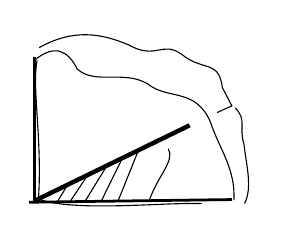
\begin{tikzpicture}[scale=0.85]
\draw[line width=1pt] (0,0)--(0,2.15);
\draw (0.06,0.02) .. controls (0.12,0.9) and (-0.04,1.7) .. (0.04,2.1);
\draw[line width=1pt] (-0.08,-0.02)--(2.95,0.02);
\draw (0.05,0.03) .. controls (0.6,-0.17) and (1.9,-0.02) .. (2.5,-0.04);
\draw (0,2.1) .. controls (0.3,2.35) and (0.5,2.25) .. (0.64,1.97)
.. controls (0.91,1.73) and (1.33,1.96) .. (1.69,1.75)
.. controls (2.0,1.5) and (2.4,1.7) .. (2.63,1.18)
.. controls (2.75,0.8) and (3.01,0.48) .. (2.98,0.01);
\draw (0.07,2.29) .. controls (0.59,2.58) and (1.01,2.5) .. (1.41,2.33)
.. controls (1.82,2.1) and (1.91,2.4) .. (2.2,2.19)
.. controls (2.54,1.92) and (2.75,2.12) .. (2.81,1.69)
--(2.95,1.42)--(2.73,1.32);
\draw (3.0,1.39) .. controls (3.18,1.21) and (3.05,1.1) .. (3.13,0.85)
.. controls (3.17,0.51) and (3.26,0.2) .. (3.14,-0.04);
\draw[line width=1.6pt] (0,0)--(2.32,1.13);
\draw (0.35,0)--(0.49,0.23);
\draw (0.54,0)--(0.8,0.39);
\draw (0.76,0)--(1.08,0.52);
\draw (1.0,0)--(1.32,0.65);
\draw (1.25,0)--(1.56,0.77);
\draw (1.72,0.02) .. controls (1.86,0.4) and (2.1,0.6) .. (2.0,0.78);
\end{tikzpicture}}

La \deleted{condition c)} impliquent que si $j'$ est
un prédécesseur de $j$, et si $k\in I$ est $\le j$
mais non $\unsure{\le|<}j'$, et s'il existe
un $i$ majoré par $k$ et $j'$, \uline{alors}
$k'=\operatorname{Inf}(k,j')$ existe, et $k'$ est
un prédécesseur de $k$.

\diagram{\begin{tikzcd}[column sep=small,row sep=small]
& j' \arrow[r,leftrightarrow,"\mathrm{préd}"'] \arrow[d,phantom,"{\unsure{\downarrow}}" description] & j \arrow[d,phantom,"{\unsure{\downarrow}}" description] \\
& k' \arrow[r,leftrightarrow] & k \\
i \arrow[uur,hook] \arrow[urr,hook] & &
\end{tikzcd}}

(Il suffit de voir que dans
un ens. ordonné de la forme $\mathcal P(\sigma)$,
les inf existent (c'est l'intersection) et si
$j'\subset j=j'\amalg\{\alpha\}$, et $k\in j$ mais non $k\subset j'$,
alors \deleted{$\unsure{k\ne k'}$} $k=k'\amalg\{\alpha\}$ avec $k'=k\cap j'$, \ldots)
\margin{$\sigma$ ens fini}

Ceci posé, considérons le diagramme
\diagram{\begin{tikzcd}
X_{j'} \arrow[r,hook] & X_j \\
X_{k'} \arrow[u] \arrow[r,hook] & X_k \arrow[u]
\end{tikzcd}}
où les flèches verticales, par l'hyp. $\unsure{1^\circ|a)}$,
sont des plongements bordants. Ceci posé, on
voit \inserted{(par b,c)} que \deleted{$X_k\longrightarrow X_{\unsure{j}}$}
$(X_k,X_{k'})\mathbin{-}(X_j,X_{j'})$
\margin{28}

\scanpage{30}
7. \uline{Stratifications} et \uline{voisinages côniques} : le pas
de récurrence.

$(X_i)_{i\in I}$, famille croissante de parties de $X$,
satisfaisant
\[
(14)\qquad\text{a) }\forall i,j\in I,\ \text{on a}\qquad
X_i\cap X_j=\bigcup_{\alpha\le i,j}X_\alpha.
\]
\inserted{$X=\bigcup_{i\in I}X_i$}

\margin{Cette condition se généralise :
aux intersections quelconques
$\displaystyle\bigcap_{i\in J}X_i=
\bigcup_{\substack{k\in I\\k\text{ minorant }J}}X_k$.}

Transversalité : un syst. de parties-bord \inserted{$B_\alpha$} de
$X$, munies de germes de cylindres associés
(mutuellement transversaux entre eux) : si on
représente les germes par des cylindres convenables
$E_{B_\alpha}$, \unsure{imposant}\inserted{\unsure{exprimant}} que les $X_i$ soient transversaux
aux $E_{B_\alpha}$ --- cela implique qu'on a
\[
E_J\cap X_i\simeq (X_{iJ}\times I^J
\qquad
\text{(induit par }E_J\simeq B_J\times I^J,
\]
avec $X_{iJ}=X_i\cap B_J$).
\deleted{\unsure{Bien sûr les}}
\margin{pour $J$ \deleted{\unsure{ensemble}} \unsure{ensemble} d'indices $\alpha$}

\deleted{\unsure{Soit}}
Soit $I_0\subset I$ une partie de $I_0$ formée
d'éléments minimaux, \deleted{et \unsure{soit}} et soit
\[
X_{I_0}=\bigcup_{i\in I_0}X_i=\coprod_{i\in I_0}X_i.
\]
\deleted{\unsure{Alors}}
La donnée d'un germe \deleted{de structure}
d'un voisinage cônique \inserted{strict} de $X_{I_0}$ équivaut à
celle d'un syst de voisinages côniques
$T_i$ ($i\in I_0$) mutuellement disjoints dans $X$. ---
celle d'un germe de voisinage cônique de $X$,
à celle d'une famille de germes de vois.
côniques des $X_i$ dans $X$.
\margin{29}

\scanpage{31}
\mspage{10}
est ``transversal'' i.e. \deleted{\unsure{si}} $\exists$ voisinages cylindriques
de $X_{j'}$ \inserted{dans $X_j$} et un de $X_{k'}$ dans $X_k$, tels que l'application
$X_k\unsure{-|\to}X_j$ induit un \deleted{\unsure{hom.}}\inserted{morphisme} sur les
cylindres (compatible avec les structures
cylindriques) et de plus
$\overline E_{k',k}=\unsure{f_{jk}|p_{jk}}^{-1}(\overline E_{j',j})$.

Système de voisinages cylindriques \deleted{associé}
\inserted{(des $X_{j'}$ dans les $X_j$)}
compatible avec une stratification : tel que
dans b, les $E_{j'j}$ ($j$ fixé, $j'$ prédécesseur)
soient compatibles. Notion correspondante
pour les germes de voisinage cylindrique.

Stratification cylindrique : stratification munie
d'une telle ``structure cylindrique'', en
termes de germes de voisinages cylindriques.

\deleted{\uline{NB} \unsure{Une}}
\uline{NB} Une stratification précylindrique \inserted{resp. cylindrique}
est \unsure{sûrement}
``équisingulier'' au sens le plus fort qu'on
puisse introduire \unsure{qui} existe.

Mais j'ai oublié une condition, que j'exigerai
de tte stratification :
\[
(0)\qquad \forall i,j\in I,\quad\text{on a}\quad
X_i\cap X_j=\bigcup_{k\le i,j}X_k
\]
\margin{\uline{NB} si $i,j$ ont pour borne inf $h$,
cela implique $X_i\cap X_j=X_h$. \unsure{même pour} \illegible{3} \unsure{c)} $\unsure{X_i\cap X_j}$.}

Corollaire : Si $X_i\cap X_j\ne\varnothing$, alors $i,j$ ont un
minorant $h$ (tel que \deleted{\unsure{le}} $X_k\ne\varnothing$\ldots)
\margin{30}

\scanpage{32}
\mspage{11}
Prenons $T_{I_0}=\coprod_{\beta\in I_0}T_\beta$ voisinage
\deleted{tubulaire}\inserted{cônique} strict
de $X_{I_0}$, supposons le strt transversal aux
$(B_i,\unsure{\mathcal E_i|E_i})$, et \deleted{aux} que les $X_i$
($i\in I^*\overset{\mathrm{def}}=I\setminus I_0$)
soient str. admissibles pour $\overline T_{I_0}$.

Notons que en vertu de (14), si $\beta\in I_0$ donc
minimal dans $I$, donc pour $i\in I$ on a
\[
(14)\qquad
X_i\cap X_\beta=
\begin{cases}
\varnothing & \text{si }\deleted{\unsure{\beta}}i\not\ge\beta\\
X_\beta & \text{sinon \unsure{i.e.} }i\ge\beta\quad(\text{ceci est trivial})
\end{cases}
\]
Soit $I_\beta$\inserted{$\subset I^*$} l'ens des $i\in I$ tels que $i>\beta$.
On a donc
\[
(15)\qquad i\in I^*\setminus I_\beta\quad\Longrightarrow\quad
X_i\cap\overline T_\beta=\varnothing
\]
(car $X_i\cap X_\beta=\varnothing$ et $X_i$ admissible pour $\overline T_\beta$),
\[
(16)\qquad i\in I_\beta\quad\unsure{\Longrightarrow|=}\quad X_i\supset X_\beta
\]
Donc on a
\[
(16')\qquad X_i\cap T_\beta
=I.\underbrace{X_i\cap\dot T_\beta}_{\dot X_i}\cup X_\beta
\]

Ainsi, le système
\[
(17)\qquad
(X,(X_i)_{i\in I},(B_\alpha,\mathcal E_\alpha)_{\alpha\in R}
(\mathcal T_\beta)_{\beta\in I_0})
\]
se reconstitue à l'aide de
\inserted{$(X_\beta)_{\beta\in I_0},$}

\deleted{
\[
(18)\quad
\left(
\underset{\substack{\parallel\\X\setminus\mathring T_{I_0}}}{X^*},
\left(\underset{\substack{\parallel\\\dot T_\beta}}{\dot X_\beta}\right)_{\beta\in I_0},
\left(\underset{\substack{\parallel\\B_\alpha\cap X^*}}{B_\alpha^*},
\underset{\substack{\parallel\\\mathcal E_\alpha\cap X^*}}{\mathcal E_\alpha^*}\right),
\left(\underbrace{(X_{\beta\alpha},\mathcal E_{\beta\alpha})}
_{=(B_{\unsure{\alpha}}^*,\mathcal E_\alpha^*)|X_\beta}\right)_{\beta\in I_0}
\right)
\]
\[
(\dot X_\beta\longrightarrow X_\beta)_{\beta\in I_0}
\]
}
\margin{31}

\scanpage{33}
\mspage{12}
\[
(18)\quad\left\{
\begin{gathered}
\underset{\substack{\parallel\\X\setminus\mathring T_{I_0}}}{X^*},
\overbrace{
\left(\underset{\substack{\parallel\\\dot T_\beta}}{\dot X_\beta},
\unsure{\mathcal E_\beta}\right)_{\beta\in I_0},
\underbrace{(B_\alpha^*,\mathcal E_\alpha^*)}
_{(B_\alpha,\mathcal E_\alpha)|X^*}{}_{\alpha\in\Lambda}
}^{\substack{\text{syst. de cylindres-bord}\\\text{transversaux}}},
\left(\underset{\substack{\parallel\\X_i\cap X^*}}{X_i^*}\right)_{i\in I^*};
(X_\beta)_{\beta\in I},
\underbrace{(B_{\beta,\alpha},\mathcal E_{\beta,\alpha})}
_{(B_\alpha,\mathcal E_\alpha)|X_\beta}
{}_{\substack{\alpha\in\Lambda\\\beta\in I_0}},\\
(\dot X_\beta\overset{p_\beta}\longrightarrow X_\beta)_{\beta\in I_0}
\end{gathered}\right\},
\]
de la façon suivante :

\margin{les $\dot X_\beta$ disjoints}
\[
(19)\quad\left\{
\begin{aligned}
\widehat X&=X^*\amalg_{\dot X=\coprod\dot X_\beta}
\underbrace{C(p=\coprod p_\beta)}
_{\deleted{\unsure{I}}\coprod_\beta C(p_\beta)},\\
T_\beta&=C(p_\beta)\\
X_\beta&\quad\text{pour }\beta\in I_0\quad\text{clair}.\\
X_i&\quad\text{pour }i\in I^*\text{ est donné par }
\deleted{\unsure{X_i=I.\dot X_i}}\\
\deleted{\unsure{X_i}}\quad X_i&=X_i^*\deleted{\unsure{\cup}}
\cup\bigcup_{\substack{\beta\in I_0\\\beta\le i\\\deleted{\unsure{i\in I_\beta}}}}
\left(I.\underbrace{\dot X_{i\beta}}
_{\substack{\parallel\mathrm{def}\\X_i^*\cap\dot X_\beta}}
\deleted{\unsure{I.(X_i^*\cap\dot X_\beta)}}\cup X_\beta\right)\\
B_\alpha&=B_\alpha^*\cup\bigcup_{\beta\in I_0}
I\underbrace{\dot B_\alpha}_{\substack{\parallel\mathrm{def}\\B_\alpha^*\cap\dot X_\beta}}\\
\mathcal E_\alpha&\quad\text{défini par }\mathcal E_\alpha^*
\text{ et les }(B_{\beta,\alpha},\mathcal E_{\beta,\alpha})
\end{aligned}\right.
\]

\uline{Conditions} sur (18)
\[
(20)\quad\left\{
\begin{array}{l}
\text{\textcircled{a} Les }\dot X_\beta\text{ disjoints}\\
\text{\textcircled{b} Chaque }\dot X_\beta\text{ transverse à }(B_\alpha^*,\mathcal E_\alpha^*)
\end{array}\right.
\]
\margin{$\Longrightarrow$ le syst. des $(\dot X_\beta,\unsure{\mathcal E_\beta})$,
$(B_\alpha^*,\mathcal E_\alpha^*)$ est \unsure{transverse}}

\inserted{\textcircled{c} Les $X_i^*$ transverses aux
$\big((\dot X_\beta,\mathcal E_\beta)_{\beta\in I_0},
(B_\alpha^*,\mathcal E_\alpha^*)_{\alpha\in\Lambda}\big)$}

\textcircled{d}
\[
(\dot X_\beta,
\underbrace{\dot B_{\beta\alpha},\dot{\mathcal E}_{\beta\alpha}}
_{\substack{\text{induit sur }\dot X_\beta\\
\text{par }(B_\alpha^*,\mathcal E_\alpha^*)}})
\longrightarrow
(X_\beta,B_{\beta,\alpha},\dot{\mathcal E}_{\beta,\alpha})
\]
est transverse
\margin{32}

\scanpage{34}
Il faut de plus des conditions qui assurent,
à partir des données (18), que $i\mapsto X_i$
est croissant, et \deleted{que} la condition (14)
$X_i\cap X_j=\bigcup_{k\le i,j}X_k$. Pour \deleted{les} exprimer ces conditions,
on introduit pour tt $\beta\in I_0$ l'ens
\[
(21)\qquad I_\beta^*=\{i\in I^*\mid i>\beta\}
\]
donc la donnée de $(I\supset\unsure{I'|I_0})$
\inserted{($I$ ens. ordonné)} équivaut à celle
de $I^*,I_0$ \inserted{(ens. ordonné \quad ens.)} et de la famille des
$I_\beta^*\subset I^*$ ($\beta\in I_0$).

Pour \deleted{vérifier}\inserted{exprimer} que \deleted{si}
$i\le j$ \inserted{(donc $j\in I^*$)} implique $X_i\subset X_j$,
on distingue les cas où $i\in I_0$\inserted{$=\beta$}
\deleted{\unsure{ou}}, où c'est
clair sur (19), et celui où $i\in I^*$ où \deleted{et} c'est
clair aussi sur (\unsure{19|17}), compte tenu de la condition
néc. évidente
\[
\text{e)}\qquad \deleted{\unsure{\forall}} i,j\in I^*,\ i\le j
\quad\Longrightarrow\quad X_i^*\subset X_j^*
\]
\deleted{Pour que}\inserted{On doit} avoir aussi, manifestement
\[
\text{f)}\qquad \unsure{j|i},j\in I^*\Longrightarrow
X_i^*\cap X_j^*=\bigcup_{k\le i,j}X_k^*
\]

Pour la relation
\[
X_i\cap X_j=\bigcup_{k\le i,j}X_k\qquad(i,j\in I)
\]
il \deleted{de} suffit de prendre le cas où $i,j$ ne
sont pas comparables. Quand un des deux
est $\in I_0$, alors cette relation \deleted{est} signifie que
$\beta\in I_0$, $i\in I^*\setminus I_\beta$, on a
$X_\beta\cap X_j=\varnothing$, ce qui résulte de (19).
\margin{33}

\scanpage{35}
\mspage{13}
Si $i,j\in I^*$, il suffit \inserted{(grâce à f))}
de vérifier que pour tt
$\beta$, on a
\[
X_i\cap X_j\cap T_\beta=\bigcup_{k\le i,j}X_k\cap T_\beta
\]
(il suffit de prouver $\subset$, car $\supset$ trivial). Si
$X_i\cap X_j\cap T_\beta=\varnothing$ c'est trivial, on peut donc supposer
$X_i\cap X_j\cap T_\beta\ne\varnothing$
\deleted{\unsure{i.e.} $X_i\cap X_j\cap$}
donc $X_i\cap T_\beta\ne\varnothing$, $X_j\cap T_\beta\ne\varnothing$
i.e. $i,j\in I_\beta$. Alors \deleted{\unsure{de}} cela résulte de
(f) induit sur $\unsure{\overline T_\beta|\dot T_\beta}=\dot X_\beta\subset X^*$,
et de la formule (19). Donc

\uline{Thm} Les systèmes (17), satisfaisant aux
conditions \deleted{\unsure{tt}} (14) des stratifications, et aux
conditions de transversalité explicitées plus
haut, équivalent aux systèmes (18), satisfaisant
aux conditions (20), en plus des conditions
e) f) exprimant que les $(X_i^*)_{i\in I^*}$ forment une
stratification de $X^*$.

8. \uline{Structure cônique sur un espace stratifié}

Pour $X$ stratifié de type $I$ par des
$(X_i)_{i\in I}$, avec des sous-espaces bordants donnés
\inserted{$(B_\alpha)_{\alpha\in\Lambda}$}
et des germes de \inserted{voisinages} cylindriques des $B_\alpha$, tels que
\deleted{\unsure{ces bords} \unsure{de} \unsure{manière}}
les $(B_\alpha)$ soient mutuellement transverses, et
transverses aux $X_i$, on va \deleted{construire} définir
\margin{34}

\scanpage{36}
par récurrence sur $\operatorname{card}I$ la notion de
\unsure{donnée|données} \deleted{de} côniques sur \deleted{cette base}
$(X,(X_i)_{i\in I},(B_\alpha,\mathcal E_\alpha)_{\alpha\in\Lambda})$.
\deleted{On procède} Si $I=\varnothing$, ce sera la structure
vide (il y en a une et une seule). Si
$I\ne\varnothing$, on prend $I_0$ ens des éléments minimaux
de $I$, et une donnée cônique sera par
définition la donnée

\textcircled{a} d'un \deleted{tube}\inserted{vois. con. strict} $\overline T_{I_0}$
de \deleted{\unsure{la somme}} $X_{I_0}=\bigcup_{\beta\in I_0}X_\beta$,
transversal aux $(B_\alpha,\mathcal E_\alpha)$ et
\deleted{\unsure{donc} admissible}
côniquement transversal aux $X_i$ ($i\in I$).
--- ce qui permet donc d'introduire les
structures (19), et en particulier

\[
(22)\qquad
X^*,\quad
\underbrace{(X_i^*)_{i\in I^*=I\setminus I_0}}
_{\text{stratification de }I^*},
\quad
\underbrace{\big((\deleted{\unsure{\mathcal E}}B_\alpha,\mathcal E_\alpha)_{\alpha\in\Lambda},
(\dot X_\beta,\mathcal E_\beta)_{\beta\in I_0}\big)}
_{\substack{\text{famille transverse}\\\text{de sous-espaces}\\
\text{bordants ``cylindrisés''}\\
\text{de }X,\ \text{transversaux}\\\text{aux }X_i}}
\]

en plus de
\[
(23)\qquad
\big((X_\beta)_{\beta\in I_0},
(B_{\beta\alpha},\mathcal E_{\beta\alpha})_{\substack{\beta\in I_0\\\alpha\in\Lambda}}\big)
\]
On doit avoir de plus : $\unsure{\infty|a}$

\textcircled{b} Une structure cônique sur (22) (ce qui
a un sens, par récurrence\ldots)
\margin{35}

\scanpage{37}
\mspage{14}

\deleted{\unsure{NB}}\quad \uline{Remarques}\quad
1) Avec des hypothèses de ``non sauvagerie'' sur la donnée initiale
\[
 (X,(X_i)_{i\in I},(B_\alpha,\mathcal E_\alpha)_{\alpha\in\Lambda}),
\]
il doit être vrai qu'il existe une structure cônique. Si la stratification
\deleted{\unsure{X}} est équisingulière le long de tout
\[
 X_i^\circ\mathrel{\mathop=^{\mathrm{déf}}}
 X_i\setminus\bigcup_{\substack{j<i\\\unsure{j\le i}}}X_j,
\]
alors il doit \(\unsure{=}\) y avoir une structure cônique équisingulière
(avec la définition ad-hoc évidente) --- il suffit de savoir construire
un tube équisingulier autour des \(X_{I_0}\) \(\cdots\)

2) A priori, si on a une suite \inserted{str.} croissante
de parties
\[
 \varnothing\subset I_0\subset I_1\cdots\subset I_n\cdots\subset I_N=I,
\]
avec \deleted{\(I_i\) formé d'él. minim.}
\inserted{\(\forall i\)} \(I_i\setminus I_{i-1}\) formé d'él. minimaux
de \(I\setminus I_{i-1}\), alors on pourrait définir
\inserted{par récurrence} une notion de structure cônique
pour cette ``filtration'' de \(I\). Mais on
peut montrer que cette notion ne dépend pas
en fait, essentiellement, de la filtration
choisie.

3) Au lieu d'une famille des \((B_\alpha,\mathcal E_\alpha)_{\alpha\in\Lambda}\),
on peut supposer donnée sur \(X\) une
stratification cylindrique \deleted{de type} (le cas envisagé
est celui où l'ens ordonné qui \deleted{\unsure{porte}}
\unsure{décrit} la stratification cylindrique est
\(\mathcal P(\Lambda)^\circ\).

\margin{36}

\scanpage{38}
Il n'y a pas de différence essentielle avec
le traitement fait ici. Plus tard on
généralisera cette notion de stratification
cylindrique (globale) en une notion de
stratification cylindrique locale --- et ce sera
la même \unsure{théorie}.

9. \uline{Description d'une} \deleted{structure}
\inserted{stratification} \uline{cônique} \uline{de type} \(I\)
(\(I\) un ordonné fini).

Pour simplifier, on prend \inserted{d'abord} le cas où on
n'a encore pas de stratification cylindrique
sur \(X\) \unsure{pour donner des ennuis}.

\deleted{\unsure{Soit}}

\margin{37}

\scanpage{39}
\mspage{15}

Stratification \deleted{\unsure{équisingulière}}\inserted{équisingulière}
de type \(I\) (\(I\) ens. ordonné fini) : présentation standart.
On suppose donnée une ``catégorie topologique modérée'' \(\mathcal M\)
(\unsure{en} un sens non précisé, pour que ça puisse être aussi celle des
espaces topologiques \(\cdots\)). La présentation est donnée
par un \inserted{contr.} foncteur
\[
 \begin{aligned}
 \Sigma:\ \operatorname{Drap}(I)&\longrightarrow\mathcal M\\
 (i_0,\ldots,i_n)&\longmapsto\Sigma_{i_0\ldots i_n}
 \end{aligned}
\]
avec les propriétés suivantes

(1) Le \deleted{\unsure{app}} morphisme
\[
 \Sigma_{i_0\ldots i_n}\longrightarrow\Sigma_{i_0,\ldots,i_p}
\]
(relatif à une inclusion de drapeaux
\(d\unsure{\hookrightarrow}d'\) telle
que \(d\) soit un segment initial de \(d'\)) est \uline{fibrant}\(^*\).

\margin{NB \inserted{on} \unsure{ne poser}
cette condition que dans le cas équisingulier.}

\margin{\(^*\) Cela est trop faible, $=$ pour
l'équisingularité --- il faut
supposer que pour \(d\) fixé, et pour
\(d'\unsure{\supset|=}d\amalg\delta\) \unsure{variable}
(où \(\delta\) est \unsure{donc}
un drapeau quelconque de
l'ens \(I'\) des \(i\in I\) \unsure{fort\(^{t}\)|fortement} \uline{\unsure{supérieur|supérieurs}}
\unsure{à} \(\unsure{\max} i_p\))
la \deleted{\unsure{famille}}\unsure{stratification}
qu'ils forment au dessus de
\(\Sigma_{d'}\) est loc. triviale.}

\deleted{(2)} (\deleted{\unsure{Enfin}} il suffit de le supposer pour
\[
 \Sigma_{i_0\ldots i_n}\longrightarrow\Sigma_{i_0\ldots i_{n-1}}
\]
)

(2) Le morphisme
\[
 \deleted{\unsure{\Sigma_{d'}}\longrightarrow\Sigma_d}
 \qquad
 \Sigma_{i_0\ldots i_n}
 \longrightarrow
 \Sigma_{i_0\ldots\widehat{i_p}\ldots i_n},
 \qquad \boxed{p\ne n}
\]
est un plongement-bord
\inserted{i.e. plongement \inserted{\unsure{bord}} cylindrique}
(NB si \(p=n\), c'est un morphisme fibrant.)

\margin{On va supposer
de plus \unsure{données|donnés}
une \deleted{\unsure{famille}} \inserted{des}
structures cylindriques
correspondantes, et \unsure{formuler}
des conditions plus fortes que
(2), \unsure{énoncées en langage}
\unsure{suivant} ---}

\uline{Cor.} Soit \(d\unsure{\hookrightarrow}d'\)
tel que \(d\) et \(d'\) aient \(\unsure{=}\)
\unsure{objt maximals}, alors
\(\Sigma_{d'}\longrightarrow\Sigma_d\) est un plongement.

\deleted{\unsure{(3)}}

\margin{38}

\scanpage{40}
\margin{\(^*\) Il suffit \unsure{pour que l'on ait} que
\(\delta=d\cap d'\) soit segment initial de \(d'\) et contienne
le plus grand élément de \(d\), ce qui dit que pour les
\(\textcircled{D}\), \(\Sigma_d-\Sigma_\delta\) est
\unsure{mono.} et \(\Sigma_{d'}-\Sigma_d\) est fibrant.
\unsure{Dans plus}}

(3) Soient \(d,d'\) deux drapeaux tels que
le dernier élément de \(d\) soit le premier élément de \(d'\)
et considérons \(d''=d\cup d'\) et le diagramme
\diagram{\begin{tikzcd}
 \Sigma_{d''}\arrow[r,hook]\arrow[d]&\Sigma_{d'}\arrow[d]\\
 \Sigma_d\arrow[r,hook]&\Sigma_i
\end{tikzcd}}
\unsure{est}
est \uline{cartésien}. (Pour \(d\) ou \(d'\)
de longueur \(0\) i.e. \unsure{n'étant} : \(\{i\}\), cette condition
est triviale.)

\margin{Il suffit de le supposer pour
\(d\) de longueur \(2\) (ou \(d'\) de longueur \(2\)).
On en déduit plus
\deleted{\unsure{la généralité que si}}
\deleted{\unsure{quelconques}}
\(d,d'\) sont deux drapeaux tels que
\inserted{\(d''=d\cup d'\)}
soit un drapeau et que
\(\delta=d\cap d'\)
\deleted{\(d\cup d'\)}
\(d''=d\amalg_\delta d'\)
\unsure{cat. ou un} \deleted{\unsure{ens}} ordonné,
\(^*\) alors
\[
 \textcircled{D}
\]
\diagram{\begin{tikzcd}
 \Sigma_{d''}\arrow[r]\arrow[d]&\Sigma_{d'}\arrow[d]\\
 \Sigma_d\arrow[r]&\Sigma_\delta
\end{tikzcd}}
est cartésien.}

\margin{De plus, il faut supposer que lorsque
\(d\) est de longueur \(2\), alors
\([\Sigma_{d'}\unsure{-|\longrightarrow}\Sigma_\delta]\) est
\uline{transverse} aux sous-espaces cylindriques \(\Sigma_d\) de
\(\Sigma_{\unsure{\delta}}\) --- et idem pour les structures cylindriques.}

\margin{(\unsure{comme au n° précédent})
On suppose de
plus que \deleted{\unsure{d'ailleurs}} si pour \(i\in I\),
\(\operatorname{Dr}(I,i)\) désigne le sous-ens ordonné
de \(\operatorname{Dr}(I)\) formé des drapeaux
\(d\) dont le dernier élément est \(i\),
de sorte que les \(\Sigma_d\) sont \(\subset\Sigma_i\),
alors les \(\Sigma_d\) forment dans \(\Sigma_i\) une
\uline{stratification précylindrique} de
type \(\operatorname{Dr}(I,i)^\circ\), ce qui s'exprime par
les conditions supplémentaires
\[
 \text{a)}\quad \Sigma_{kj}\cap\Sigma_{\ell j}=\varnothing
 \quad\text{si }k,\ell\unsure{\le}j\text{ sont des noncomparables}.
\]
\[
 \text{b)}\quad
 \Sigma_{i_0\ldots i_n}
 =\Sigma_{i_0i_n}\cap\Sigma_{i_1i_n}\cdots
 \cap\Sigma_{i_{n-1}i_n}
 \qquad\text{dans }\Sigma_{i_n}
\]
\[
 \left(\Longleftrightarrow\
 \Sigma_d\cap\Sigma_{d'}=
 \begin{cases}
 \varnothing&\text{si }d\cup d'\text{ \unsure{pas un drapeau}}\\
 \Sigma_{d\cup d'}&\text{sinon}
 \end{cases}\right)
\]
c) L'intersection dans b) est transversale.
On suppose plus précisément, \unsure{choisis|choisies} des structures
cylindriques \unsure{qui rendent transversales}
\(\Sigma_{ij}\) \(\unsure{(i<j)}\).}

Cela nous donne un procédé \unsure{canonique} pour
reconstruire les \(\Sigma_d\), à isom. \inserted{can.} près,
quand on connaît les \(\Sigma_i,\Sigma_{ij}\)
\inserted{\((i<j)\)} et les morphismes
\diagram{\begin{tikzcd}
 \Sigma_{ij}\arrow[r,hook]\arrow[d]&\Sigma_j\\
 \Sigma_i&
\end{tikzcd}}
\deleted{Pour}
(NB \unsure{que}
la flèche verticale est fibrante, et l'horizontale
un morphisme-bord). Pour avoir les
morphismes de transition entre les
\(\Sigma_d\) (construits par récurrence sur \(\operatorname{long}d\),
les \(0\) et \(1\) étant déjà donné) il faut se donner
les morphismes
\[
 \underbrace{\Sigma_{ij}\mathbin{\times_{\Sigma_j}}\Sigma_{jk}}
 _{\mathrel{\mathop=^{\mathrm{déf}}}\Sigma_{ijk}}
 \longrightarrow\Sigma_{i,k}
\]
satisfaisant aux conditions

\margin{39}

\scanpage{41}
\mspage{16}

La donnée des \(\Sigma_i\) équivaut à la donnée d'un
\[
 \Sigma_*\in\mathcal M\qquad
 \left(\Sigma_*=\coprod\Sigma_i\right)
\]
et d'une partition de type \(I\) de \(\Sigma_*\) i.e. d'un morphisme
\[
 \Sigma_*\longrightarrow I_{\mathcal M}.
\]
Celle des \(\Sigma_{ij}\) équivaut à celle
d'un objet \(\Sigma_{**}\) \deleted{\unsure{et|de}} \unsure{au} dessus de \(I\times I\)
\deleted{\(\operatorname{Drap}_{\unsure{1}}(I)\)}
\deleted{\(\unsure{I\times I}\)}
(on pose \(\Sigma_{ij}=\varnothing\) si \(i\not\le j\),
\(\Sigma_{ii}=\Sigma_i\)).

La donnée des
\diagram{\begin{tikzcd}
 \Sigma_{ij}\arrow[r,hook]\arrow[d]&\Sigma_j\\
 \Sigma_i&
\end{tikzcd}}
équivaut à celle de deux morphismes ``source'' et ``but''
\diagram{\begin{tikzcd}
 \Sigma_{**}\arrow[r,"\underline b"]\arrow[d,"\underline s"']&\Sigma_*\\
 \Sigma_*&
\end{tikzcd}}
compatibles avec les \(\operatorname{pr}_1\) et \(\operatorname{pr}_2\)
de \(I\times I\) dans \(I\)
(\deleted{\uline{NB} \unsure{le cas}}
car la bigraduation \inserted{de type \(I\)}
de \(\Sigma_{**}\) est déduite de \deleted{\unsure{celle}}
\unsure{graduation} de type \(I\) de \(\Sigma_*\), et des
\(\underline b\) et \(\underline s\)) ---
\unsure{où} \(\underline b\) est \inserted{\unsure{loc.\(^{t}\)}}
un morphisme bord (i.e. est une
immersion bord) et \(\underline s\) est une fibration.

On a de plus \unsure{a}
\[
 \underline{\unsure{i|\iota}}:\ \Sigma_*\unsure{-|\longrightarrow}\Sigma_{**}
\]
``morphisme identité'', dont le composé avec \(\underline b\) et
\(\underline s\) est l'identité. La donnée des
\(\Sigma_{ijk}\unsure{-|\longrightarrow}\Sigma_{ik}\) revient à

\margin{40}

\scanpage{42}
une \uline{application} \uline{composition}, et l'axiome à
formuler pour avoir une extension \deleted{en}
\inserted{des \(\Sigma_i,\Sigma_{ij}\)}
en des \(\Sigma_{i_0\ldots i_n}\), est que cette composition
(qui est compatible avec les unités, \unsure{manifestement},
par construction) soit une structure de
\uline{\(\mathcal M\)-catégorie}\(^*\). \deleted{\unsure{une}}
Donc la donnée de \(\Sigma\) satisfaisant (3)
équivaut à celle d'un Cat-objet de \(\mathcal M\),
au dessus de la catégorie \unsure{discrète} \(I_{\mathcal M}\) :
\[
 \Sigma_{\mathcal M}\longrightarrow I_{\mathcal M}.
\]

\margin{\(^*\) En fait, c'est un objet
\uline{ordonné} de \(\mathcal M\), et
\(\Sigma_{i_0\ldots i_n}\) s'identifie à l'ens des drapeaux
\[
 x_{i_0}\le x_{i_1}\le\cdots\le x_{i_n}
\]
de \(\Sigma_*\), au dessus des drapeaux
\(i_0-\cdots-i_n\) de \(I\).
Donc pour vérifier \unsure{(cf. p. 15, marge)}
\[
 \Sigma_{i_0\ldots i_n}
 =\Sigma_{\unsure{i_0i_1|i_0i_n}}\cap\cdots
 \cap\Sigma_{\unsure{i_0i_n}}
\]
il suffit de le vérifier pour \(n=2\), i.e.
\[
 \Sigma_{\unsure{ijk}}=\Sigma_{ik}\cap\Sigma_{jk},
\]
ce qui signifie que pour
tt \(z\in\Sigma_k\), \(\Sigma_*\unsure{-|\longrightarrow}I\) induit
\diagram{\begin{tikzcd}[column sep=large]
 \Sigma_*(z)\arrow[r,hook]\arrow[d,equal]&I(k)\arrow[d,equal]\\
 \{x\in\Sigma_*\mid x\le z\}&\{i\in I\mid i\le k\}
\end{tikzcd}}
qui est tel que l'ordre de \(\Sigma(z)\)
soit \uline{induit} par celui de \(I(k)\).
\deleted{Cela signifie}}

A l'aide de ces données, je vais
construire un espace stratifié de type \(I\),
sans utiliser en fait \deleted{aucune des hypothèses}
\inserted{les \deleted{\unsure{deux}} conditions}
(1) \deleted{et (2)}, la condition (2) n'intervenant
que sous la forme plus faible que
\[
 \Sigma_{i_0\ldots i_n}
 -\Sigma_{i_0\ldots\widehat{i_p}\ldots i_n}\qquad(p\ne n)
\]
est un plongement \deleted{bord}
(\unsure{si on ne veut pas construire} les structures côniques
relatives à l'espace stratifié obtenu).

Je considère pour ceci les couples
\deleted{\(d,d'\)} \((d\subset d')\) de deux drapeaux,
\deleted{\unsure{une}} tels que
\(d\) \deleted{de \(d'\)} ne soit pas cofinal dans \(d'\).
(Pour \(d'\) \inserted{\(=\{i_0,\ldots,i_n\}\)}
\deleted{de longueur \(n\)}
il y a donc \(2^n\) choix possibles pour \(d\)).

\margin{41}

\scanpage{43}
\mspage{17}

On considère que cette donnée équivaut à celle d'une
suite d'inclusions de drapeaux
\[
 d_1\subset d_2\cdots\subset d_p\subset d_{p+1}=d'
 \qquad(p=\operatorname{long}.d')
\]
dont chacun est un segment initial strict de
le \deleted{\unsure{précédent}}\inserted{suivant}.
Ceci donne donc \deleted{des filt} une
suite de projections
\[
 \Sigma_{d'}=\Sigma_{d_{\unsure{p+1|p-1}}}\unsure{-|\longrightarrow}\Sigma_{d_p}
 \unsure{-|\longrightarrow}\cdots\unsure{-|\longrightarrow}\Sigma_{d_2}
 \unsure{-|\longrightarrow}\Sigma_{d_1}
\]
dont on considère le mapping-cône simultané
qu'on désigne par
\[
 C_\Sigma(d_1,d_2,\ldots,
 \underset{\substack{\Vert\\d'}}{d_{\unsure{p+1|p-1}}})
\]
ou aussi par \(\unsure{\mathbb C|C}_{\Sigma,d,d'}\).
On veut déterminer les
morphismes \inserted{\unsure{entre eux}} de transition naturels entre
\[
 C_{\Sigma,d,d'}.
\]

\margin{NB \(d\) est l'ens des
éléments maximaux
des \(d_1,\ldots,d_p\)}

\margin{On reviendra sur cette
\uline{construction} \uline{plus tard}.
Elle n'est pas tellement
utile finalement \(\cdots\)}

\uline{10.} Reprenons la description \unsure{Ab ovo|ab ovo}
(dans le cas \(\mathcal M=(\mathrm{Top})\), pour fixer les idées
--- c'était le contexte adopté au début de ces notes).

\deleted{On}
On a un espace topologique
\figure{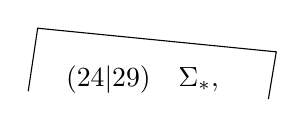
\begin{tikzpicture}[baseline]
 \node at (1.45,0) {\((\unsure{24|29})\quad\Sigma_*,\)};
 \draw (0,-0.15) -- (0.12,0.65) -- (3.15,0.35) -- (3.05,-0.25);
\end{tikzpicture}}
muni d'une relation d'ordre
\[
 \Sigma_{**}\subset\Sigma_*\times\Sigma_*
\]
ayant un graphe fermé, et tel que
\[
 \Sigma_{**}\xrightarrow{\operatorname{pr}_2=\mathrm{but}}\Sigma_*
\]
soit une \deleted{plongement}\inserted{immersion} --- plus

\margin{\textcircled{10}}
\margin{42}
